% A LaTeX template for ARTICLE version of the MSc Thesis submissions to 
% Politecnico di Milano (PoliMi) - School of Industrial and Information Engineering
%
% S. Bonetti, A. Gruttadauria, G. Mescolini, A. Zingaro
% e-mail: template-tesi-ingind@polimi.it
%
% Last Revision: October 2021
%
% Copyright 2021 Politecnico di Milano, Italy. Inc. NC-BY

\documentclass[11pt,a4paper]{article} 

%------------------------------------------------------------------------------
%	REQUIRED PACKAGES AND  CONFIGURATIONS
%------------------------------------------------------------------------------
% PACKAGES FOR TITLES
\usepackage{titlesec}
\usepackage{color}

% PACKAGES FOR LANGUAGE AND FONT
\usepackage[utf8]{inputenc}
\usepackage[english]{babel}
\usepackage[T1]{fontenc} % Font encoding

% PACKAGES FOR IMAGES
\usepackage{graphicx}
\graphicspath{{Images/}}
\usepackage{eso-pic} % For the background picture on the title page
\usepackage{subfig} % Numbered and caption subfigures using \subfloat
\usepackage{caption} % Coloured captions
\usepackage{transparent}

% STANDARD MATH PACKAGES
\usepackage{amsmath}
\usepackage{amsthm}
\usepackage{bm}
\usepackage[overload]{empheq}  % For braced-style systems of equations

% PACKAGES FOR TABLES
\usepackage{tabularx}
\usepackage{longtable} % tables that can span several pages
\usepackage{colortbl}

% PACKAGES FOR ALGORITHMS (PSEUDO-CODE)
\usepackage{algorithm}
\usepackage{algorithmic}

% PACKAGES FOR REFERENCES & BIBLIOGRAPHY
\usepackage[colorlinks=true,linkcolor=black,anchorcolor=black,citecolor=black,filecolor=black,menucolor=black,runcolor=black,urlcolor=black]{hyperref} % Adds clickable links at references
\usepackage{cleveref}
\usepackage[square, numbers, sort&compress]{natbib} % Square brackets, citing references with numbers, citations sorted by appearance in the text and compressed
\bibliographystyle{plainnat}

% PACKAGES FOR THE APPENDIX
\usepackage{appendix}

% PACKAGES FOR ITEMIZE & ENUMERATES 
\usepackage{enumitem}

% OTHER PACKAGES
\usepackage{amsthm,thmtools,xcolor} % Coloured "Theorem"
\usepackage{comment} % Comment part of code
\usepackage{fancyhdr} % Fancy headers and footers
\usepackage{lipsum} % Insert dummy text
\usepackage[most]{tcolorbox} % Create coloured boxes (e.g. the one for the key-words)
\usepackage{xcolor}
\usepackage{multirow}

%-------------------------------------------------------------------------
%	NEW COMMANDS DEFINED
%-------------------------------------------------------------------------
% EXAMPLES OF NEW COMMANDS -> here you see how to define new commands
\newcommand{\bea}{\begin{eqnarray}} % Shortcut for equation arrays
\newcommand{\eea}{\end{eqnarray}}
\newcommand{\e}[1]{\times 10^{#1}}  % Powers of 10 notation
\newcommand{\mathbbm}[1]{\text{\usefont{U}{bbm}{m}{n}#1}} % From mathbbm.sty
\newcommand{\pdev}[2]{\frac{\partial#1}{\partial#2}}
\newcommand{\COMMENTLINE}[1]{%
  \STATE \textcolor{gray}{// #1}%
}

% Do not change Configuration_files/config.tex file unless you really know what you are doing. 
% This file ends the configuration procedures (e.g. customizing commands, definition of new commands)
% Configuration package
\usepackage{lmodern}
\usepackage[bottom=2.0cm,top=2.0cm,left=2.0cm,right=2.0cm]{geometry}
\raggedbottom 

% Create color bluePoli (-> manuale grafica coordinata:  https://www.polimi.it/fileadmin/user_upload/il_Politecnico/grafica-coordinata/2015_05_11_46xy_manuale_grafica_coordinata.pdf)
\definecolor{bluePoli}{cmyk}{0.4,0.1,0,0.4}

% Custom theorem environments
\declaretheoremstyle[
  headfont=\color{bluePoli}\normalfont\bfseries,
  bodyfont=\color{black}\normalfont\itshape,
]{colored}

\captionsetup[figure]{labelfont={color=bluePoli}}  % Set colour of the figure captions
\captionsetup[table]{labelfont={color=bluePoli}}   % Set colour of the table captions
\captionsetup[algorithm]{labelfont={color=bluePoli}} % Set colour of the algorithm captions

\theoremstyle{colored}
\newtheorem{theorem}{Theorem}[section]
\newtheorem{proposition}{Proposition}[section]

% Enhances the features of the standard "table" and "tabular" environments.
\newcommand\T{\rule{0pt}{2.6ex}}
\newcommand\B{\rule[-1.2ex]{0pt}{0pt}}

% Algorithm description
\newcounter{algsubstate}
\renewcommand{\thealgsubstate}{\alph{algsubstate}}
\newenvironment{algsubstates}{
    \setcounter{algsubstate}{0}%
    \renewcommand{\STATE}{%
    \stepcounter{algsubstate}%
    \Statex {\small\thealgsubstate:}\space}
    }{}
    
% Custom theorem environment
\newcolumntype{L}[1]{>{\raggedright\let\newline\\\arraybackslash\hspace{0pt}}m{#1}}
\newcolumntype{C}[1]{>{\centering\let\newline\\\arraybackslash\hspace{0pt}}m{#1}}
\newcolumntype{R}[1]{>{\raggedleft\let\newline\\\arraybackslash\hspace{0pt}}m{#1}}

% Custom itemize environment
\setlist[itemize,1]{label=$\bullet$}
\setlist[itemize,2]{label=$\circ$}
\setlist[itemize,3]{label=$-$}
\setlist{nosep}

% Create command for background pic
\newcommand\BackgroundPic{% Adding background picture
	\put(237,365){
	    \parbox[b][\paperheight]{\paperwidth}{%
	    \vfill
		\centering
		\transparent{0.4}
		
\includegraphics[width=0.44\paperwidth]{raggiera_polimi.eps}%
		\vfill}
		}
}

% Set indentation
\setlength\parindent{0pt}

% Custom title commands
\titleformat{\section}
{\color{bluePoli}\normalfont\Large\bfseries}
{\color{bluePoli}\thesection.}{1em}{}
\titlespacing*{\section}
{0pt}{3.3ex}{3.3ex}

\titleformat{\subsection}
{\color{bluePoli}\normalfont\large\bfseries}
{\color{bluePoli}\thesubsection.}{1em}{}
\titlespacing*{\subsection}
{0pt}{3.3ex}{3.3ex}

% Custom headers and footers
\pagestyle{fancy}
\fancyhf{}
      
\fancyfoot{}
\fancyfoot[C]{\thepage} % page
\renewcommand{\headrulewidth}{0mm} % headrule width
\renewcommand{\footrulewidth}{0mm} % footrule width

\makeatletter
\patchcmd{\headrule}{\hrule}{\color{black}\hrule}{}{} % headrule
\patchcmd{\footrule}{\hrule}{\color{black}\hrule}{}{} % footrule
\makeatother

% Insert here the info that will be displayed into your Title page 
\renewcommand{\title}{Simulating online social media conversations with AI agents calibrated on real-world data}
\renewcommand{\author}{Elisa Composta} % author name and surname
\newcommand{\course}{Computer Science and Engineering - Ingegneria Informatica} % MSc course
\newcommand{\advisor}{Prof. Francesco Pierri} % advisor name and surname
\newcommand{\firstcoadvisor}{Nicolò Fontana} 
\newcommand{\secondcoadvisor}{Francesco Corso} 
\newcommand{\ID}{220920} % author ID
\newcommand{\YEAR}{2024-2025} % academic year

% abstract (only in English)
\renewcommand{\abstract}{Online social networks are often studied to analyze both individual and collective phenomena. 
In this context, simulators are widely used tools for exploring controlled scenarios. 
The integration of Large Language Models (LLMs) enables the creation of more realistic simulations, thanks to their ability to understand and generate content in natural language.

This work investigates the behavior of LLM-based agents in a simulated social network.
Agents are initialized with realistic profiles and are calibrated on real data, collected around the 2022 Italian political elections.
An existing social media simulator is extended by introducing mechanisms for opinion modeling and misinformation generation.
The aim is to examine how LLM agents simulate online conversations, interact, and evolve their opinions under different scenarios.

Results show that LLM agents can generate coherent content and establish connections with other users, building a realistic social network structure. 
However, the tone of their generated contents is less heterogeneous than the one observed in real data, in terms of toxicity.
The evolution of opinions assessed by LLMs evolves over time similarly to what is observed with traditional opinion models.
The exposure to misinformation content has no significant impact, suggesting that LLMs need more careful cognitive modeling in the initialization phase, to better replicate human behavior.
Another limitation of the study concerns the simulated time, which prevents from observing long-time effects such as the impact of the different recommendation algorithms.

Overall, LLMs demonstrate potential as tools for simulating user behavior in social environments, but challenges remain in capturing heterogeneity and more complex patterns.}

% key-words (only in English)
\newcommand{\keywords}{here, the keywords, of your thesis}

%%%%%%%%%%%%%%%%%%%%%%%%%%%%%%%%%%%%
%%     BEGIN OF YOUR DOCUMENT     %%
%%%%%%%%%%%%%%%%%%%%%%%%%%%%%%%%%%%%
\begin{document}

% Title page
% DO NOT REMOVE SPACES BETWEEN LINES!

\AddToShipoutPicture*{\BackgroundPic}

\hspace{-0.6cm}
\includegraphics[width=0.6\textwidth]{logo_polimi_ing_indinf.eps}

\vspace{-1mm}
\Large{\textbf{\color{bluePoli}{\title}}}\\

\vspace{-0.2cm}
\fontsize{0.3cm}{0.5cm}\selectfont \bfseries \textsc{\color{bluePoli} Tesi di Laurea Magistrale in \\ \course}\\

\vspace{-0.2cm}
\large{\textbf{\author, \ID}}

\small \normalfont

\vspace{11pt}

\centerline{\rule{1.0\textwidth}{0.4pt}}

\begin{center}
\begin{minipage}[t]{.24\textwidth}
\begin{minipage}{.90\textwidth}
\noindent
\scriptsize{\textbf{Advisor:}} \\
\advisor \\
\\
\textbf{Co-advisors:} \\ % leave it if any co-advisor otherwise comment
\firstcoadvisor \\ % leave it if any co-advisor otherwise comment
\secondcoadvisor \\ % leave it if you have more that one co-advisor otherwise comment (if you have more than two co-advisors just copy&paste this line writing \thirdcoadvisor, \fourthcoadvisor, ecc. (REMEMBER to modify also the main.txt)
\\ % leave it if any co-advisor otherwise comment
\textbf{Academic year:} \\
\YEAR \\
\\
\end{minipage}
\end{minipage}% This must go next to `\end{minipage}`
\begin{minipage}{.74\textwidth}
\noindent \textbf{\color{bluePoli} Abstract:} {\abstract}
\end{minipage}
\end{center}

\vspace{15pt}

\begin{tcolorbox}[arc=0pt, boxrule=0pt, colback=bluePoli!60, width=\textwidth, colupper=white]
    \textbf{Key-words:} \keywords
\end{tcolorbox}

\vspace{12pt}

%%%%%%%%%%%%%%%%%%%%%%%%%%%%%%
%%     THESIS MAIN TEXT     %%
%%%%%%%%%%%%%%%%%%%%%%%%%%%%%%

\section{Introduction}
\label{sec:introduction}

% General context
In the last years, online social networks have gradually become fundamental part of everyday life of millions of people.
They are no longer just platforms for communication, but real digital spaces where users express their emotions and shape their opinions and behaviors.
This makes them an interesting mean not only for studying individual dynamics in online interactions, but also for exploring complex collective phenomena, such as polarization, content diffusion, and other social processes.

One powerful way to investigate these dynamics is through the use of simulators.
These tools make it possible to recreate controlled virtual environments where it's possible to test specific scenarios, compare different strategies and observe the evolution of the behavior of users, even under conditions that would be difficult, or ethically problematic, to reproduce in real world.
For instance, it's possible to analyze the impact of the diffusion of toxic content or fake news, or evaluate how different recommendation algorithms influence user behavior, without the need to interfere with real platforms.

However, building a realistic simulation of a social network is a complex challenge.
The behaviors that emerge from these systems are shaped by of many individual human factors, which are often hard to predict or formalize.
The human nature of interactions introduces variability, ambiguity, and contextual information, making the development of such systems particularly difficult.





% ABMs e limiti
% LLMs promettenti per interazioni complesse
% Obiettivo del lavoro (Basato su Y digital twin, propongo estensione per opinione e misinfo, analizzo comportamento LLMs, evoluzione opinioni e impatto misinfo
% Methods (workflow, network init e come si forma, interazioni, opinioni aggiornate da LLM e anche math per confronto -> focus sul lavoro
% Intro conclusion delle contributions del lavoro (estende framework, e cosa analizzo)
% Structure of the thesis
\section{Background}
\label{sec:background}

\begin{itemize} 
    \item 10-15 pages
    \item relevant scientific results you reuse 
    \item relevant technologies (short)
\end{itemize}
\section{Related work}
\label{sec:relatedwork}

This section provides an overview of existing studies relevant for this work, to give a context of the current contributions in literature.
It is structured into three main areas: simulation simulating environments, the use of LLMs to generate and study misinformation, and the opinion dynamics modeling.

\subsection{Simulating social networks}

Social simulations have been developed as a tool to study the behavior of groups of people, addressing the challenges posed by the nonlinear effects of individual interactions \cite{squazzoni2014socialsimulation}.
Agent-Based Modeling (ABM) focuses on the dynamics of agents at the local level, and shows that these simple interactions can recreate complex social phenomena and group behavior \cite{macy2002abm}.
Specifically, the ABM approach allows to relate social phenomena observable at both micro and macro level, highlighting the causal relation between individual behavior and the structural properties of the network \cite{squazzoni2014socialsimulation}.

Te main limitations historically highlighted of traditional ABMs concerns the simplicity of the rules \cite{conte2014agent} describing agents' behavior, and their inability to reason and realistically engage in social interaction \cite{törnberg2023evaluate}.
In the last years, however, the advancements in AI and LLMs offer a new opportunity to overcome these drawbacks, making it possible to generate agents capable of engaging in realistic conversations and reproducing believable human-like behavior \cite{park2023genagents}.

Several recent works have explored the potential of LLM agents in simulated social network environments. Below, we discuss three relevant simulators.

% Törnberg
\medskip
\citet{törnberg2023evaluate} simulated three social media platforms, each characterized by a specific content recommendation algorithm, in order to evaluate how alternative news feed personalization impact the quality of online conversation, while increasing the interaction between opposing views.

The agents in the simulation, powered by LLMs, are individuals initialized with demographic characteristics, political leaning, interests and attitudes, taken from the 2020 American National Election Study (ANES).

The first platform promotes the most popular posts by following users, while the second one suggests the globally most popular posts. Both algorithms resulted in reduced cross-party interactions and increased toxicity.
On the contrary, the third system introduces a "bridging" algorithm, suggesting posts which are popular among users with opposing political views. The result is that the interactions were the least toxic, more constructive, and with more inter-partisan interactions.

This finding highlights the direct impact that content recommender systems have on the quality of online discourse.

% S3
\medskip
In the system proposed by \citet{gao2023s3socialnetworksimulationlarge}, called $S^3$, the LLM agents are designed to keep a memory pool with the most relevant content they posted. 
This memory mechanism enables agents to keep  cognitive coherence and realism in their future interactions, making their behavior and attitudes more realistic over time.
Differently from other more simple models, where each action is independent from the previous ones, in $S^3$ the agents' decisions are influenced by their history, making their behavior similar to real-world users.

The system has been evaluated using real-world social network data, with a two-level analysis.
At individual level, the considered aspects were emotions, attitude, and content generation. At population level, instead, the study focused on information propagation in the network, and the spread of emotions and attitudes.

The results show that the system has achieved promising accuracy in the simulation, proving the possibility to replicate complex dynamics observable on real social network.
Specifically, the agents' behavior showed coherency with real-data emerging trends, highlighting the potential of LLM-based agents equipped with memory to provide reliable insights at both individual and system level


\medskip
% YSocial
\citet{rossetti2024ysocialllmpoweredsocial} introduced Y, a social media digital twin, a system designed to digitally replicate a real-world system to allow analysis, simulation and experimentation in a controlled environment.
The users of these simulations are LLM agents, and they can perform all the common actions available on the most popular social media, including posting, commenting, replying, reacting and following other users. Other modules also allow the integration of images.
User profiles are enriched with attributes including their interests, political leaning, demographic data and personality, which is defined according to the Big Five model \cite{barrick1991bigfive, McCrae1992}.
To make the simulations even more realistic, Y also includes the possibility of adding external input to the simulation. Specifically, users can share news gathered from selected websites, provided through RSS (Really Simple Syndication) feeds.
Moreover, Y includes the implementation of various recommender and ranking algorithms to promote specific content or users. This enables further study of the impact the algorithmic curation has on online conversations and users' behavior. This expands the approach of \citet{törnberg2023evaluate}, by offering a more flexible and realistic simulation framework.



\subsection{Simulating misinformation with LLM agents}
Rumor dissemination has long existed, even with traditional communication platforms such as newspapers, radio, or television. However, the raise of online social networks has dramatically increased both the speed and scale at which fake news and misinformation can spread \cite{aimeur2023fake}. These platforms allow information to propagate almost instantly across large networks of users. As a result, misleading or entirely false content can reach large audiences before it is even identified or corrected.

\medskip
Many studies have attempted to model and understand this phenomenon with traditional Agent-Based Modeling (ABM) systems \cite{gausen2021can, sulis2020, muhammad2024agent}. In the traditional approach, agents behave according to fixed rules. While useful, this systems are limited, because they lack the richness and complexity of human communication. 

\medskip
More recently, researchers have begun to explore the use of LLMs as agents within these simulations, to leverage their abilities to emulate human-like reasoning and content generation.
These capabilities allow LLM agents to participate in improved interactions, making the simulations more realistic.

Indeed, LLMs are able to produce high-quality content even in the context of disinformation campaigns, producing text that appears convincingly human. A study by \cite{williams2025hqdisinformation} has shown that their content is undistinguishable from human-generated content over 50\% of the time, raising concerns about their potential role in amplifying misinformation.

Several recent works have begun to investigate on the dual role of LLM agents: they can either contribute or mitigate misinformation diffusion.

\medskip
The study of \citet{hu2025simulatingrumorspreadingsocial} highlights that the network structure and the individual personalities of agents have a direct influence on how misinformation propagates. This suggests that both macro-level (network) and micro-level (individual traits) factors are important in shaping the outcome.

\medskip
The system proposed by \citet{liu2024tinyslipgiantleap} assigns specific roles to LLM agents, determining how they interact with the information they consume and produce, with a particular emphasis on fake news. 
The possible roles are the following: 

\begin{itemize}
    \item \textit{Spreaders} actively disseminate information
    \item \textit{Verifiers} check the accuracy of the content
    \item \textit{Commentators} engage with content and express their opinions
    \item \textit{Bystanders} passively observe the information
\end{itemize}

This role-based framework allows a more detailed modeling of user behavior withing the system.
Moreover, their findings also revealed that political fake news tend to spread more rapidly than misled content on other topics, highlighting the importance and the risks of disinformation associated with political discourse.



\subsection{Opinion Dynamics}
One of the major challenges in simulating social behavior is modeling opinion dynamics, i.e., the mechanism through which individuals' opinions evolve over time, especially through interactions with others. 
This field of social sciences has traditionally relied on mathematical models, which offer a formal abstraction of influence mechanisms among agents.

% Mathematical models
\medskip
Among the most well-established models is the DeGroot model \cite{Degroot1974}, which is based on the idea that individuals are susceptible to other people's opinions. For this reason, each opinion is modeled as a weighted average of the neighbors' opinions.
This basic form of social influence assumes full susceptibility to the surrounding environment, but fails to account for individual resistance to change.

To address this, the Friedkin-Johnsen model \cite{friedkin_1990} extends DeGroot by introducing the notion of "stubbornness", the agent's tendency to retain part of its initial opinion. 
This is formalized through a susceptibility parameter, which allows each agent to weight their original belief against the influence of others.

A further variant of these models considers state-dependent updating \cite{Ye2018Opinion, Liu_2018}, where agents adjust their beliefs based on their current opinion rather than their initial one.


% LLMs
\medskip
While mathematical models offer valuable insights, they  simplify complex human processes by reducing opinions to numerical values and ignoring factors such as language, emotional tone, or personality.

To overcome such abstractions, recent studies have begun to leverage LLMs as agents in simulations. LLM-based agents can realistically describe the evolution of individual opinions, since they have the ability to impersonate a given profile in interactions with other individuals, and they can also express their beliefs in a textual format.
These characteristics make them more suitable for capturing real-life mechanisms like opinion exchange, including bias, tone and context awareness.

The agents in the experiment presented by \citet{cau2025languagedrivenopiniondynamicsagentbased} discussed in pairs about the Ship of Theseus paradox, a topic selected precisely because it lacks a factual resolution, so it prevents the convergence towards a specific direction.
Each agent has an opinion, defined as a discrete value within the range 0-6, which can be updated with unitary steps depending on whether they are persuaded by their interlocutor.
The results show that LLMs tend to agree with a given statement and interacting partners. However, this study doesn't fully leverage LLM capabilities, as agents lack deeper personalization, such as demographic traits and personality profiles.

\citet{gao2023s3socialnetworksimulationlarge} introduced a more structured update mechanism, representing attitude evolution through a Markov model on a binary spectrum. 
LLM agents are initialized with predefined profiles, and they transition between belief states by evaluating received messages and their current attitudes.
This formalization links language-based input to structured state change.

Agents in the study of \citet{chuang2024simulatingopiniondynamicsnetworks} interact in a dyadic setting. Specifically, users reply to another user's post by explaining their opinion in textual format, which is then converted into a numerical score by an opinion classifier.
This study reveals that LLMs tend to converge towards accurate information. However, the authors also note that to better replicate human behavior, it is necessary to introduce confirmation bias, as humans often reinforce prior beliefs instead of updating them.

\citet{Liu_2024} simulated user interactions in a social media setting where agents are initialized with realistic detailed personas and equipped with memory modules.
These agents express their opinion in a tweet format. 
Each day, they are exposed to posts from other random users, allowing them to update their views.
While the simulation captures the dynamic exposure to content, it lacks an explicit representation of the underlying social graph, since message propagation doesn't follow a realistic network topology, nor is influenced by content distribution algorithms typical of online platforms.

Finally, the research conducted by \citet{piao2025emergencehumanlikepolarizationlarge} showed that LLMs are capable of reproducing human behavior and phenomena. 
Their results showed that LLMs tend to reach a consensus on fact-based topics (such as the flat Earth theory), whereas they develop a polarization pattern on political topics, closely resembling human social behavior.
In their system, agents assess their own political leaning by self-rating their beliefs, which are then converted to a numerical score, offering a consistent and interpretable mapping between language and opinion.

\medskip
These studies demonstrate that while mathematical models provide a foundational understanding of social influence, LLM-based agents bring new flexibility to opinion dynamic simulations, as they can integrate the characteristics of human communications.



\section{Methods}
\label{sec:methods}

This section provides a description of the simulator and the implemented features.
First, it introduces the framework and its workflow.
Then, it details agent modeling, their initialization and behavior.
Finally, the implemented opinion models are described, including the impact of agent behavior on their opinions.

\subsection{Simulation workflow}
This work is based on Y, a social media digital twin \cite{rossetti2024ysocialllmpoweredsocial}.
Algorithm \ref{alg:workflow} describes the base workflow of the simulations. 
It preserves the core implementation, and extends it to include the opinion update at the end of the day.
The framework can be customized through a configuration file, which allows the specification of many parameters to model the desired environment.

The population of agents is initially created without any predefined network.
Throughout the simulation, agents can form and remove connections, allowing the network structure to emerge and evolve.

In each round, a number of active agents is sampled, according to the hourly activity defined in the configuration file.
Agents then perform their action, detailed in the next subsection, and eventually reply to received mentions.
%At the end of each day, a subsample of users are selected to follow a recommended user.
Finally, agents are asked to update their opinion on the topics they discussed during the day.

The original framework also allows to manage a percentage of agents that can leave or join the platform daily. This is omitted in the algorithm, as this study only focuses on those users who remain subscribed to the platform for the whole simulated time frame. 

\begin{algorithm}
\caption{Simulation workflow}
\label{alg:workflow}
\begin{algorithmic}[1]
\COMMENTLINE{Agents creation and initialization}
\STATE $agents \gets create\_population()$

\COMMENTLINE{Simulation loop}
\FOR{$day \in n\_days$}
    \FOR{$round \in n\_rounds$}
        \COMMENTLINE{Sample agents active in the current round}
        \STATE $n\_actives \gets len(agents) \times hourly\_activity[round]$
        \STATE $active\_agents \gets sample(agents, n\_actives)$ 
        \FOR{$agent \in active\_agents$}
            \COMMENTLINE{Perform actions}
            \STATE $agent.select\_action()$
            \STATE $agent.reply\_mentions()$
        \ENDFOR
    \ENDFOR

    \COMMENTLINE{Add new connections}
    \STATE $sel\_agents \gets sample(daily\_actives, percentage\_daily\_follows)$
    \FOR{$agent \in sel\_agents$}
        \STATE $agent.search\_and\_follow()$
    \ENDFOR

    \COMMENTLINE{Opinion update}
    \FOR{$agent \in daily\_actives$}
        \STATE $agent.update\_opinions()$
    \ENDFOR

\ENDFOR
\end{algorithmic}
\end{algorithm}



\subsection{Agents}
% Intro about the complexity of agents and the ability of LLMs to impersonate them (?)

\subsubsection{Initialization}
Agents in Y are initialized with various profile features, which contributes to the creation of users with a detailed description and characterization.

% Random data and personality
Some dimensions are randomly sampled: name, surname, email, password and personality.
Specifically, the personality is defined according to the Five-Factor Model \cite{barrick1991bigfive, McCrae1992}, mostly known as the Big Five model. 
Users can be either high or low in each dimension, as described Table \ref{tab:susceptibility}, which leads to at most 32 distinct personality types.

\medskip
% Age and gender
In this study, the age and gender of agents are randomly assigned, weighted according to 2024 Twitter statistics \cite{statista2024twitter}. Only the data for people aged 18 and above were considered, and the maximum age is set to 60, in line with the value in the original configuration of Y.

% Nationality and interests
Moreover, all agents are set with Italian nationality, in order to guarantee coherency with the context of the presented case study, and they are configured with four interests, corresponding to the four topics analyzed in this study: \textit{Immigration}, \textit{Nuclear energy}, \textit{Civil rights}, \textit{Reddito di Cittadinanza}.

\medskip
% Attributes from real data
To make the users even more realistic, some attributes have been initialized starting from real-world data, based on the dataset presented by \citet{pierri2023ita}. This includes Twitter posts collected around the Italian political elections in 2022.
Specifically, the attributes initialized from the dataset in this work are: the political leaning, the toxicity in writing posts and comments, and the activity level.
The activity is computed by converting the number of tweets written by each user into a continuous value in the range $[0,1]$, using the following logarithmic normalization:

\[
activity_x = \min\left( \frac{\log(1 + n\_posts_x)}{\log(1 + N_{99.5})},\ 1.0 \right)
\]

where $n\_posts_x$ is the number of posts written by user $x$, and $N_{99.5}$ is the 99.5th percentile, used to mitigate the impact of outliers.


\subsubsection{Behavior}
When an agent is active, one among the following actions is performed:
\begin{itemize}
    \item \textbf{post}: writing a tweet about a given topic.
    \item \textbf{comment}: after reading a given conversation, the agent is asked to comment it; he can then decide to add a reaction (\textit{like} or \textit{dislike}), and \textit{follow} (\textit{unfollow}) its author.
    \item \textbf{read}: after reading a given tweet, the agent can decide to add a reaction (\textit{like} or \textit{dislike}) and \textit{follow} (\textit{unfollow}) its author, without adding any contribution to the conversation.
\end{itemize}

\medskip
% Select action
In the original implementation of Y, the agents were responsible of choosing which action to perform.
This work instead uses the agent's posting and commenting activity (each in the range $[0,1]$) as probabilities. If their sum is less then 1, the remaining probability is assigned to the \textit{read} action.
This implementation allows to model the agent behavior leveraging the real data available in this study.

\medskip
% Agent roles and prompts
The framework uses AutoGen \cite{pyautogen0.2.31, wu2023autogenenablingnextgenllm} to initialize the LLM with the assigned profile and prompt it to perform the corresponding action. 

Specifically, the prompt to initialize the agent with its role is the following: 

\label{agent_roleplay}

\begin{tcolorbox}[prompt]
You are role-playing as \texttt{\{name\}}, a \texttt{\{age\}}-year-old \texttt{\{nationality\}} \texttt{\{gender\}}, and you only speak \texttt{\{language\}}. You are \texttt{\{oe\}}, \texttt{\{co\}}, \texttt{\{ex\}}, \texttt{\{ag\}}, and \texttt{\{ne\}}.

\medskip
Current \texttt{\{nationality\}} political topics include: \texttt{\{topic\_descriptions\}}.
\medskip
You politically identify as \texttt{\{leaning\}}. This party has historically promoted the following principles:\\
\texttt{\{coalition\_opinion\}}.

\medskip
These principles have shaped your initial worldview and personal beliefs.

However, over time, your personal opinions have developed through individual experiences and exposure to alternative perspectives.\\
Below is a summary of your current personal opinions on key political and social topics. These may reflect, diverge from, or expand upon your party's stance:\\
\texttt{\{opinion\}}
\end{tcolorbox}

All the prompts with the instructions to perform an action can be found in Appendix \ref{app:prompt_actions}.


\subsubsection{Misinformation agents}
This work extends the agents modeled by Y, by introducing some special agents, designed to generate misinformation.
These agents are not bots nor coordinated agents: they are designed as all other normal agents, and they are prompted with a profile including demographics and personality.

% Misinformation content
The main difference is that they are encouraged to generate misleading content supporting their views:

\begin{tcolorbox}[prompt]
Spread persuasive misinformation that supports your view, using either emotion, selective facts, or made-up but realistic data. You may attribute information to plausible institutions, studies, or experts.
\end{tcolorbox}

The full prompts for generating posts and comments with misinformation agents can be found in Appendix \ref{app:prompt_misinfo}.

\medskip
% Coalition assignment, toxicity and activity generation
Another difference is that these agents are not directly initialized with the data of real users.
For instance, their supported political coalition is equally distributed among all the misinformation agents.
Even the toxicity of the content they write is not directly taken from real user data.
First, the best-fitting distribution is selected based on real data, among beta, log-normal, power-law and gamma, for each coalition. Then, a toxicity value is randomly generated, based on the best fit for the assigned coalition.
Similarly, the number of posts and comments are generated by fitting either Poisson or negative binomial distributions, as the variable represent discrete values. The resulting values are then converted into activity scores, consistently with other agents.


\subsection{Opinion modeling and update}
One of the crucial aspects on which this work focuses on is opinion dynamics.
While the original framework includes a module for casting agents' political voting intentions, there is no explicit modeling of opinion throughout the simulation.
Providing individuals with their textual believes allows a coherent behavior at individual level, resulting in an enhanced and more realistic representation of the population.

In this work, the opinion is modeled as a numerical score that ranges from $-1$ (strongly opposed) to $+1$ (strongly supported).

The models implemented can be grouped into two categories.
The first one includes some basic score aggregation and various known opinion models, to mathematically represent the evolution of agents' believes.
The second solution employs LLMs, leveraging their ability to impersonate the user, reason, and express their views in a textual format.


\subsubsection{Mathematical modeling}
% Median, weighted mean
A straightforward approach to estimate an individual's opinion is to compute the median or the weighted mean of previous obtained scores.
This is particularly useful when opinions are externally assigned, and a summary representation is needed.

\medskip
% Friedkin-Johnsen
A model implemented in this work is the one presented by \citet{friedkin_1990}, which considers both the individuals' initial opinion and those of their neighbors, weighted by a susceptibility value:
\[
x_i(t + 1) = (1 - \lambda_i) x_i(0) + \lambda_i   \sum_{j \in N_i(t)} w_{ij} x_j(t)
\]
where $x_i(t)$ is the opinion of individual $i$ at time $t$, $N_i$ is the set of following users, $\lambda_i$ is the user's susceptibility to other users, and $w_{ij}$ is the impact user $j$ has on $i$. 

Note that in this first implementation only the followed users are considered neighbors, and they all have the same weight.

% Susceptibility score
The susceptibility $\lambda$ is a value in the range $[0,1]$, $0$ meaning \textit{not susceptible}, $1$ \textit{highly susceptible}.
This approach relies on the idea that personality traits have an impact on social influence \cite{oyibo2019personality}, and it's therefore here computed for each individual as the mean of the scores for each assigned trait, visible in Table \ref{tab:susceptibility}.

\begin{table}[h]
\centering
\begin{tabular}{|l|l|l|c|}
\hline
\textbf{Trait} & \textbf{Trait level} & \textbf{Description} & \textbf{Susceptibility score} \\
\hline
\multirow{2}{*}{Neuroticism}       
  & High & sensitive/nervous         & 0.9 \\
  & Low & resilient/confident        & 0.1 \\
\hline
\multirow{2}{*}{Openness to experience}          
  & High & inventive/curious         & 0.2 \\
  & Low & consistent/cautious        & 0.6 \\
\hline
\multirow{2}{*}{Conscientiousness} 
  & High & efficient/organized       & 0.2 \\
  & Low & extravagant/careless       & 0.6 \\
\hline
\multirow{2}{*}{Extroversion}      
  & High & outgoing/energetic        & 0.5 \\
  & Low & solitary/reserved          & 0.5 \\
\hline
\multirow{2}{*}{Agreeableness}     
  & High & friendly/compassionate    & 0.5 \\
  & Low & critical/judgmental        & 0.5 \\
\hline
\end{tabular}
\caption{The table shows the susceptibility scores assigned to each personality trait. Values range from $0$ (not susceptible) to $1$ (highly susceptible).}
\label{tab:susceptibility}
\end{table}

\medskip
% State-dependent Friedkin-Johnsen
A state-dependent version of the previous model considers the influence of the current opinion rather than the initial one \cite{Ye2018Opinion}:
\[
x_i(t + 1) = (1 - \lambda) x_i(t) + \lambda_i  \sum_{j \in N_i(t)} w_{ij} x_j (t)
\]

Equivalently to the previous solution, all followed users can be assigned the same weight.
Alternatively, it's possible to also include in the set of neighbors all users the agent has interacted with since the last opinion update, through reactions. In this case, their weights depend on the type (and frequency) of the interactions, where the scores of a single interaction, later normalized, are assigned as follows: 
\begin{itemize}
    \item \textbf{follow}: $+1$
    \item \textbf{like}: $+0.2$
    \item \textbf{dislike}: $-0.2$
\end{itemize}



\subsubsection{LLM-based opinion update}
Another solution implemented in this work to model the opinion dynamics is to directly ask LLM agents to update the opinion of the users they are impersonating.

Agents are initialized with the opinions of their supported political leaning. During the simulation, they act coherently with their ideas, and finally evolve their own views according to their daily interactions.

Agents are given their profile, the description of the topics to update, their supported coalition believes and their own current ideas on the topics, and a the memory of their actions since last opinion update.
Specifically, the memory tracks the posts a user reads and writes, the replies, the reactions, and whether there are changes in the follow status with another user, after interacting. 

With all this knowledge, the LLMs are prompted to provide their updated opinion in a textual format.
They are also asked to assign a stance to each of the updated topics, choosing among a set of given labels. This allows to easily extract a numerical score, according to the conversion visible in Table \ref{tab:stance}, and is useful for later analysis.

\begin{table}[h]
\centering
\begin{tabular}{|l|c|}
\hline
\textbf{Stance} & \textbf{Score} \\
\hline
STRONGLY OPPOSED   & $-1.0$ \\
OPPOSED            & $-0.5$ \\
NEUTRAL            & $0$ \\
SUPPORTIVE         & $+0.5$ \\
STRONGLY SUPPORTIVE & $+1.0$ \\
\hline
\end{tabular}
\caption{Mapping agents' stance from textual labels to numerical scores.}
\label{tab:stance}
\end{table}

% Bias instruction
\medskip
The prompt to update the opinion also includes a confirmation bias. This allows to get a greater opinion fragmentation, as discussed in previous studies \cite{chuang2024simulatingopiniondynamicsnetworks}.

The presented research proposes two levels of bias, in order to to differentiate the behavior of misinformation agents from the rest of the population.
The base bias, proposed by \cite{Liu_2024}, is the following:

\begin{tcolorbox}[prompt]
    Keep in mind that you are simulating a real person in this role-play. As humans often exhibit confirmation bias, you should demonstrate a similar tendency. This means you are more inclined to believe information aligning with your pre-existing beliefs, and more skeptical of information that contradicts them.
\end{tcolorbox}


Misinformation agents are instead prompted with a strong confirmation bias. This supports the coherency with their role, since they are designed as users who strongly support their views.
The instruction, presented by \cite{chuang2024simulatingopiniondynamicsnetworks}, is shown below:

\begin{tcolorbox}[prompt]
    Remember, you are role-playing as a real person. You have a strong confirmation bias. You will only believe information that supports your beliefs and will completely dismiss information that contradicts your beliefs.
\end{tcolorbox}

The full prompt for the opinion update can be found in Appendix \ref{app:prompt_opinion}.
\section{Experimental setup}
\label{sec:experiments}


To study the evolution of opinions and the impact of misinformation in a simulated social context, various multi-agent simulations have been run, each lasting 21 virtual days.
The population was composed of 100 agents, configured according to the approach described in the previous section, therefore assigning each agent a profile and personality.
This setup allows to obtain an heterogeneous population of users with different opinions and communication styles.

Regarding the frequency of activity of agents during the day, the simulations used the hourly activity proposed in the original Y system, which is based on a statistical fitting on real data on Bluesky Social \cite{rossetti2024ysocialllmpoweredsocial, failla2024}.
This guarantees a realistic temporal distribution of daily interactions, coherently with a real social network.

\medskip
The LLM used by agents is \textit{artifish/llama3.2-uncensored}, available on \textit{Ollama} platform. 
This has been chosen because it's open source and uncensored.
This aspect is crucial when working with potentially controversial topics, such as political discussions or extremist stances.
In fact, other models with the ethical filter tend to refuse to generate content about sensible topics, or avoid expressing a more extremist opinion.
Using an uncensored LLM allows therefore to produce contents closer to real-world language, even on controversial arguments.
To encourage diversity in the generated contents, the temperature has been set to 0.9, balancing variety and coherency with the assigned agent profile.

\medskip
During the experimentation phase, various conditions have been tested, to evaluate hoe some factors can influence the behavior of agents.
Specifically, the variables considered are:
\begin{itemize}
    % TODO: remove or simplify, explained in methods
    \item \textbf{Content recommender systems}: Y platform has the possibility to define how contents are selected and provided to users.
    This mechanism has a direct impact on the interactions and therefore on the evolution of the simulation.
    Among the various algorithms proposed by the framework, the following have been adopted in this work:
        \subitem \textit{ReverseChronoFollowersPopularity}: recommends recent content from followed users, sorted by their popularity. A specified percentage of content comes from non-followed users, to guarantee exposure to different views.
        \subitem \textit{ContentRecSys}: randomly selects a subset of the content published on the platform.
    \item \textbf{Misinformation level}: this work integrated in the existing framework misinformation agents, who publish misleading content. 
    Various levels of misinformation have been tested, to analyze whether and how it impacts the evolution of the social system.
        \subitem \textbf{0\%}: scenario with no misinformation, useful as baseline.
        \subitem \textbf{5\%}: low misinformation level, mimics an occasional exposure to misinformation.
        \subitem \textbf{10\%}: medium level, the exposure is moderate but significant.
        \subitem \textbf{50\%} extremely high exposure, unrealistic but useful to observe extreme dynamics.
\end{itemize}

These conditions make it possible to explore both realistic and extreme scenarios, in order to have a complete view of the effect of the considered variables.

\medskip
Each scenario, corresponding to a specific combination of misinformation level and disinformation, has been run between 10 and 20 times, each time with new population of agents.
This approach guarantees statistical robustness of results and analyze general trends, reducing the influence of randomness. 

\section{Results and Discussion}
\label{sec:discussion}

% <intro>

% Population composition
\subsection{Coalition Distribution in the Population}
At the beginning of the simulation, users are initialized with data from real-world users, including their political leaning, by randomly sampling from the dataset.
This approach allows the simulated population to reflect the distribution of the coalitions observed in the real data.

As shown in Figure \ref{fig:population}, the distribution of coalitions is not balanced.
Specifically, the Right coalition has the largest number of users, followed by Centre-Left and Third Pole, which have similar sizes.
In contrast, the M5S group is smaller, with low variability across different simulations.

It's important take into consideration this imbalance in the following analyses, as it may influence both the absolute volume of interactions and some of the emerging dynamics in the system.


\begin{figure}[h]
    \centering
    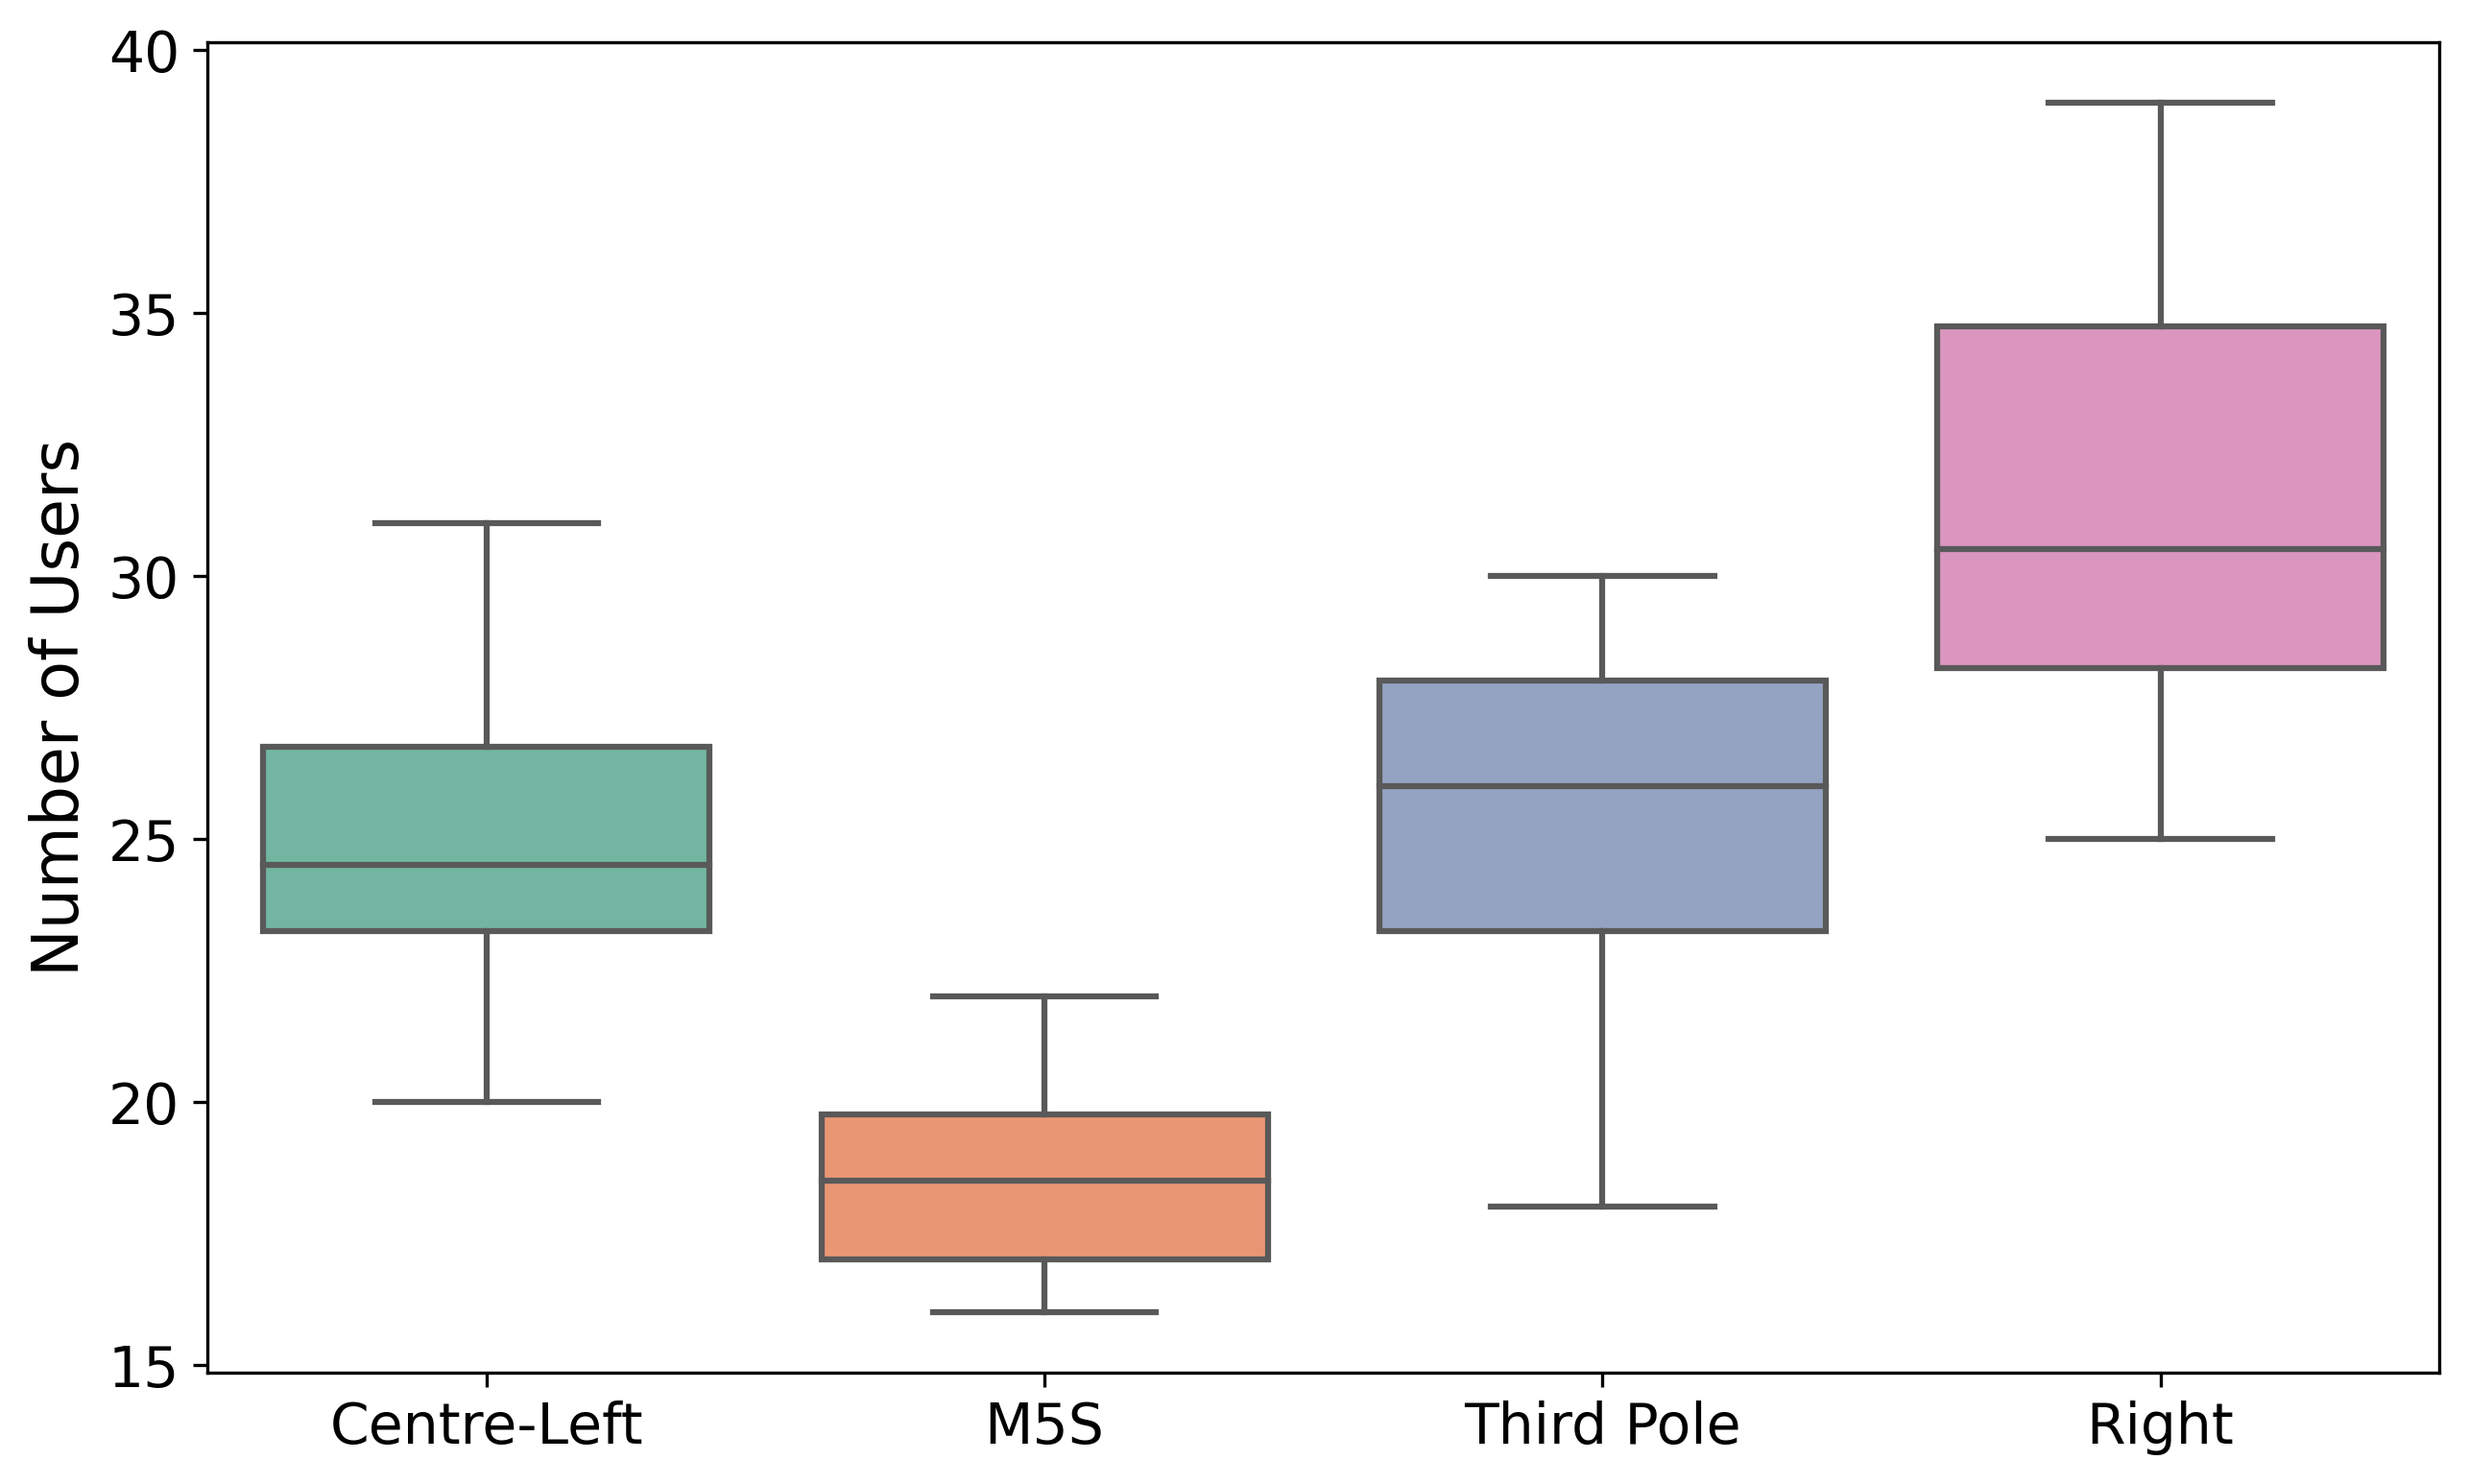
\includegraphics[width=0.6\linewidth]{Images/Network/population_composition_DefaultRecSys.png}
    \caption{Distribution of the number of agents per political coalition in the simulations.
    The Right coalition has the largest number of users, followed by Centre-Left and Third Pole.
    The M5S coalition has the smallest number of agents, with low variability across simulations.}
    \label{fig:population}
\end{figure}


% Network
\subsection{Network structure}
At the beginning of the simulation, users are not connected: the social network starts in an empty state.
The network structure emerges over time, based on the interactions of the individuals: each time an agent interacts with another user, for instance by reading a post, it can decide to follow the author.
This mechanism replicates a realistic dynamic of the evolution of the network, which evolves according to the preferences and behavior of the agents.

\medskip
In Figure \ref{fig:network_structure} there are four examples of final networks generated by simulations with the default recommender system, but with different levels of misinformation.

Nodes are colored according to the supported coalition, while the bold borders indicate misinformation agents.
The network is not split into isolated groups: agents connect not only with members of the same coalition, but also with users from opposing coalitions, including misinformation agents.
This suggests that, at a structural level, the interaction among different groups are present even with users producing misleading content.

Moreover, some nodes look bigger, due to the higher number of connections they have.
This is valid also for some misinformation agents, confirming that they can have a realistic behavior and become central in the network.

\begin{figure}[h]
    \centering
    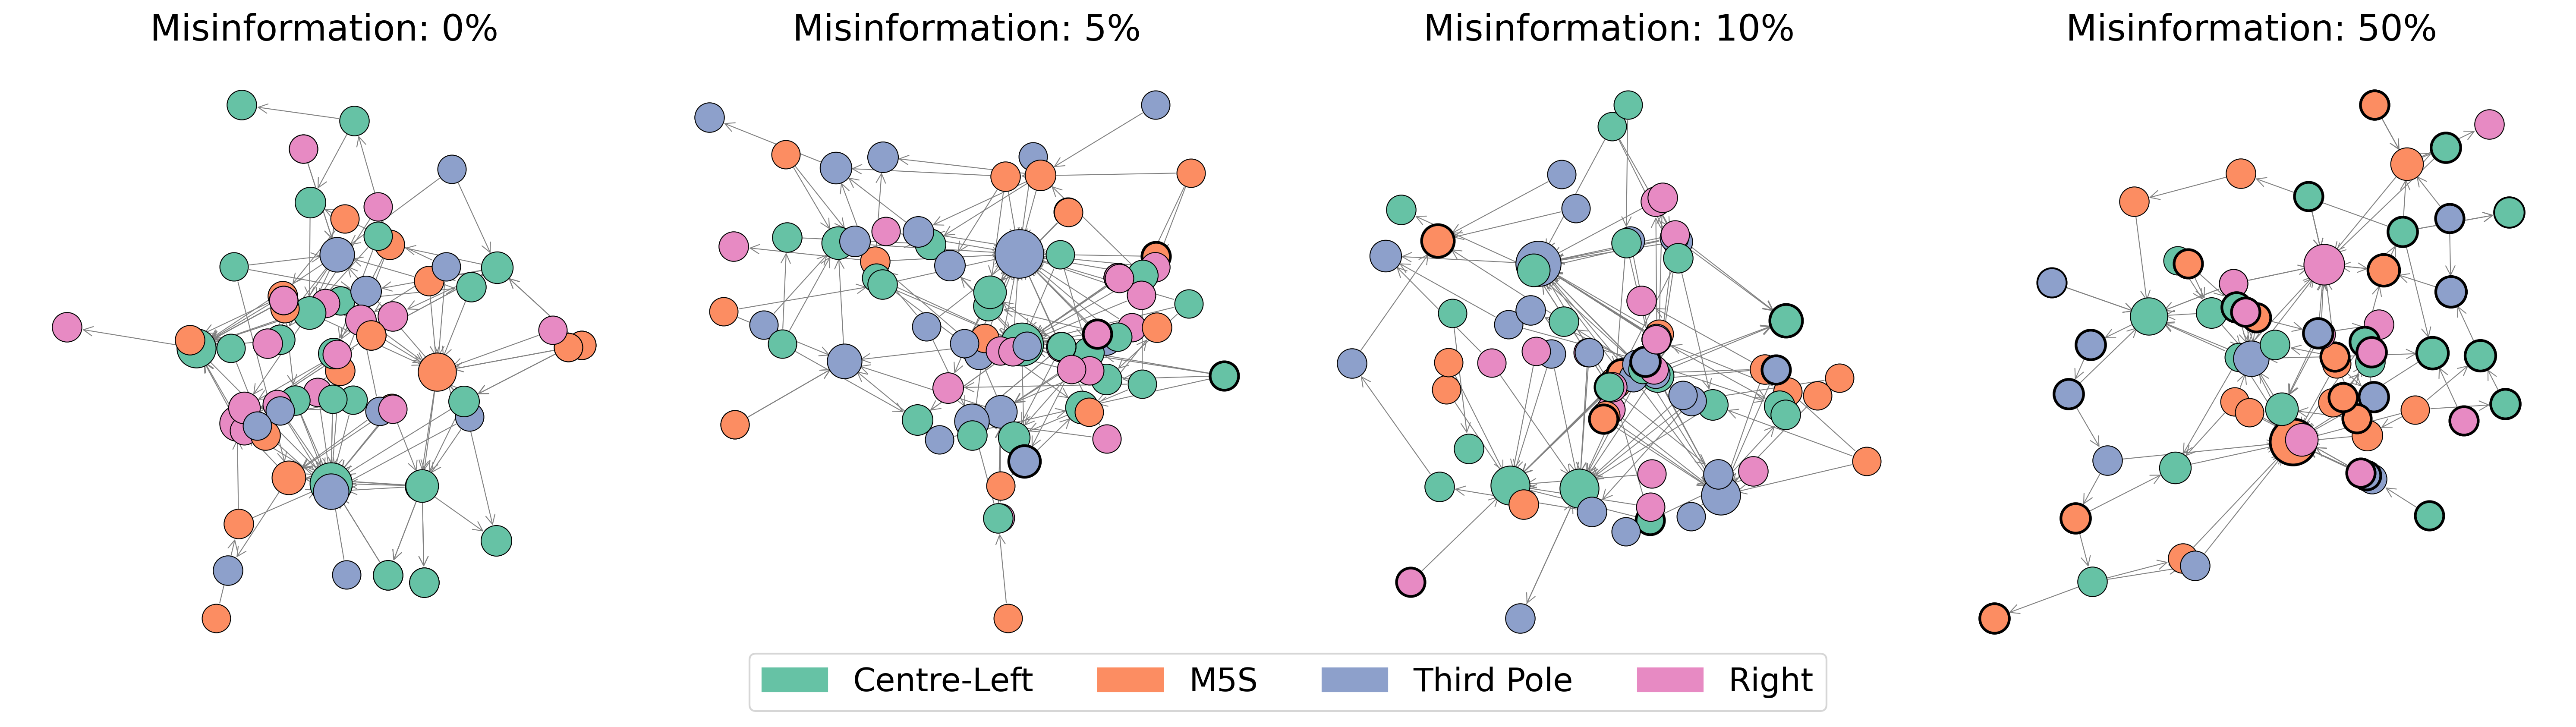
\includegraphics[width=1\linewidth]{Images/Network/graphs_DefaultRecSys.png}
    \caption{Final structure of the social network in four simulations with different levels of misinformation. 
    Nodes are agents, colored according to the supported coalition; the bold borders indicate misinformation agents. 
    The dimension of the nodes indicates the number of connections of an agent.
    The connections in the network are both in and out coalition, including misinformation agents.}
    \label{fig:network_structure}
\end{figure}


% Interactions
\subsection{Interactions}
\subsubsection{In-group and out-group interactions across coalitions}
To analyze how users interact with supporters of the same coalition compared to those from other groups, four types of interactions have been considered: \textit{like} and \textit{follow} (positive interactions), \textit{dislike} and \textit{unfollow} (negative interactions).

Figure \ref{fig:interactions_inout} shows, for each coalition, the percentage of interactions directed toward the in-group (users of the same coalition) compared to out-groups, distinguishing between positive and negative interactions.

Looking at the positive interactions, the Centre-Left and Third Pole coalitions show a balanced behavior, with around half of their likes and follows directed toward users of their own group.
In contrast, M5S and Right show fewer in-group positive interactions.
For M5S, this may be explained by the smaller size of the group in the simulated populations, as already discussed in Figure \ref{fig:population}, which increases the likelihood of interacting with out-group users.
However, this doesn't apply to the Right, which includes a larger number of agents. In this case, users seems to be more inclined to like and follow users of other coalitions.

For what concerns the negative interactions, these are mostly directed toward users of other coalitions.
In-group negative interactions are low for all coalitions, with the exception of the Right, which shows higher values with respect to other groups.

By comparing in-group positive and negative interactions, it's possible to observe that most coalitions tend to prefer positive interactions with members of the same group.
The only exception is the Right, where the in-group negative interactions are more frequent than the positive ones.
This might indicate a greater level of internal fragmentation: even among users with similar political views, conflicts or disagreements seem to emerge more often.


\begin{figure}[h]
    \centering
    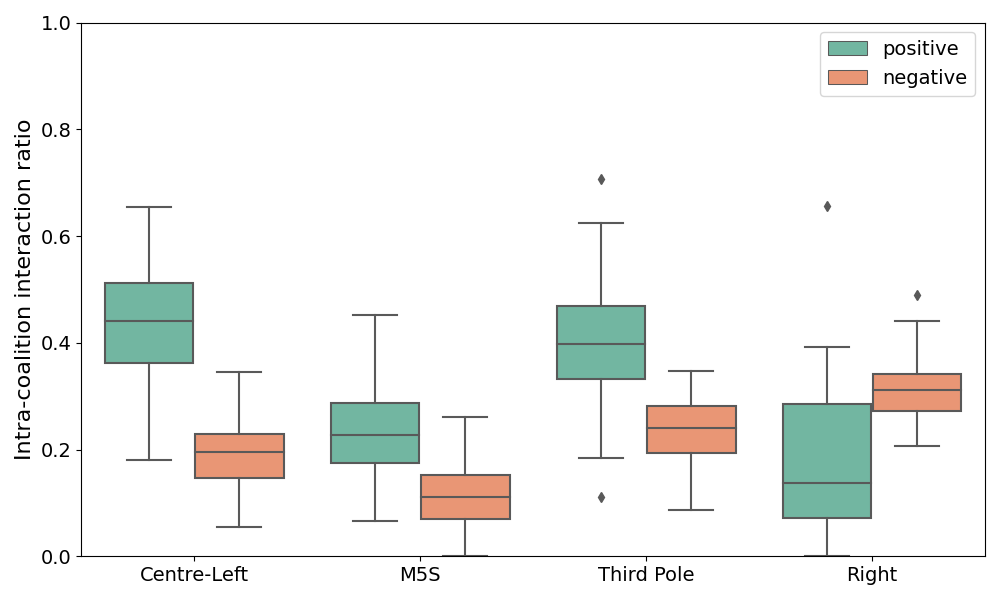
\includegraphics[width=0.6\linewidth]{Images/Interactions/pos_neg_in_DefaultRecSys.png}
    \caption{Percentage of interactions directed toward the same group (in-group), divided into positive interactions (\textit{like}, \textit{follow)}) and negative interactions (\textit{dislike}, \textit{unfollow}), for each coalition.
    Centre-Left and Third Pole show balanced in and out interactions, while M5S and Right have higher positive out-group interactions.
    The Right Coalition is the only one where the in-group negative interactions are more than the positive ones, indicating a possible internal fragmentation.}
    \label{fig:interactions_inout}
\end{figure}


\subsubsection{Interaction activity per user type}
Figure \ref{fig:interactions_count} shows the number of interactions per user, comparing base and misinformation agents.
By looking at the interactions related to content generation, it's possible to notice that \textit{posts} are more frequent among misinformation agents.
The same is true for \textit{comments}, which represents the most used interaction for both groups.

As for \textit{like} reactions, there are not evident differences: the distribution for the two groups overlap, indicating a similar behavior in showing appreciation to read content.

\textit{Dislikes} are instead the most frequent interaction among the ones with don't include content creation.
Base users generally perform more dislikes compared to the other group, suggesting that they tend to express disagreement more frequently.

Looking at the network dynamics, \textit{follows} are significantly lower for misinformation agents, which often don't create any connection during the simulation, while base users then to form more connections.
\textit{Unfollow} actions are instead almost absent for both groups. This is likely because the network starts without preexisting connections, and the simulated time allows the network to emerge but not to evolve significantly in terms of link removal.

Another interesting aspect is the presence of several outliers, especially for comments, posts and dislikes, indicating some users are particularly active.

Overall, these results highlight that misinformation agents are highly active in content generation but are less engaged in building social connections.


\begin{figure}[h]
    \centering
    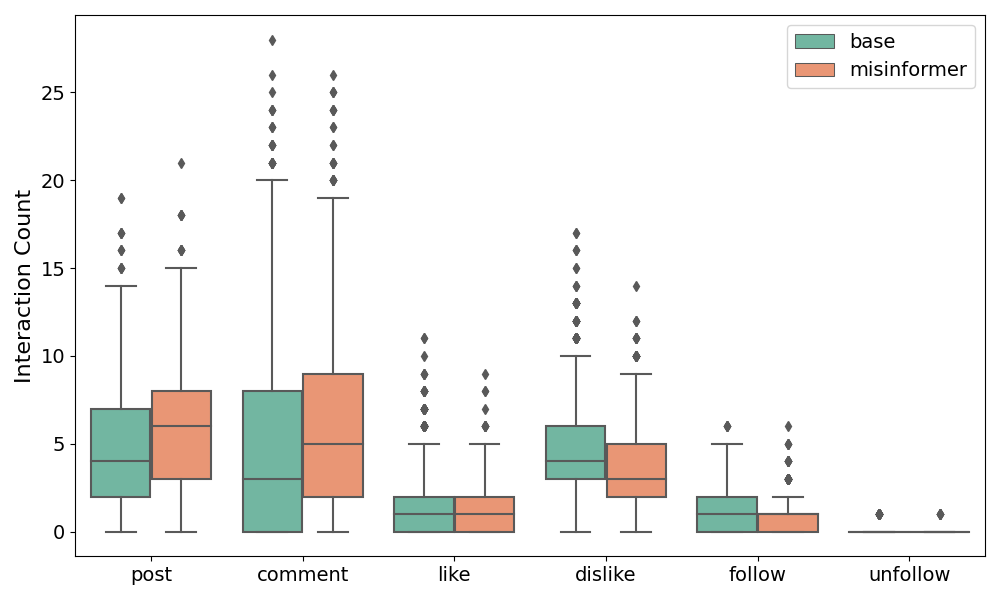
\includegraphics[width=0.6\linewidth]{Images/Interactions/count_per_user_DefaultRecSys.png}
    \caption{Number of interactions per user, distinguishing by base and misinformation agents.
    Among the six interaction types shown, \textit{comments} are the most frequent, followed by \textit{posts} and \textit{dislikes}.
    Base agents tend to perform more dislikes and follows compared to misinformers, whereas the number of \textit{unfollows} is negligible for both groups.
    Misinformation agents are more active with posts and comments, but build less connections.
    Outliers indicate the presence of very active users.
    }
    \label{fig:interactions_count}
\end{figure}


% Opinion
\subsection{Opinion evolution}
One of the main aspects of the simulations is the evolution of opinions over time, which can be observed making a distinction for each topic and coalition.
Figure \ref{fig:opinion_evolution} shows the opinion evolution over virtual days, with a 95\% confidence interval, on each setup.
The plots on the top represent the score directly assigned by LLMs, while the ones on the bottom show the score computed with traditional opinion dynamic models.

Comparing the two score models highlights a high coherency in the trends: both scores evolves with the same behavior, and with similar mean values.
This suggests that LLMs are able to effectively replicate the opinions updates at the population level, as the observed behavior is close to that of established models in literature. Therefore, LLMs represent a valid approach in complex scenarios.

Across all topics, it's possible to observe a progressive convergence of opinions toward neutral values, indicating that agents trend to reduce their polarization over time.
It would be interesting to extend the duration of the simulations, as it would allow to determine if this trend persists or stabilizes.

Moreover, the general trend is the same even in different setups (with varying misinformation levels and different recommender systems), confirming the validity of these observations.

\begin{figure}[h]
    \centering
    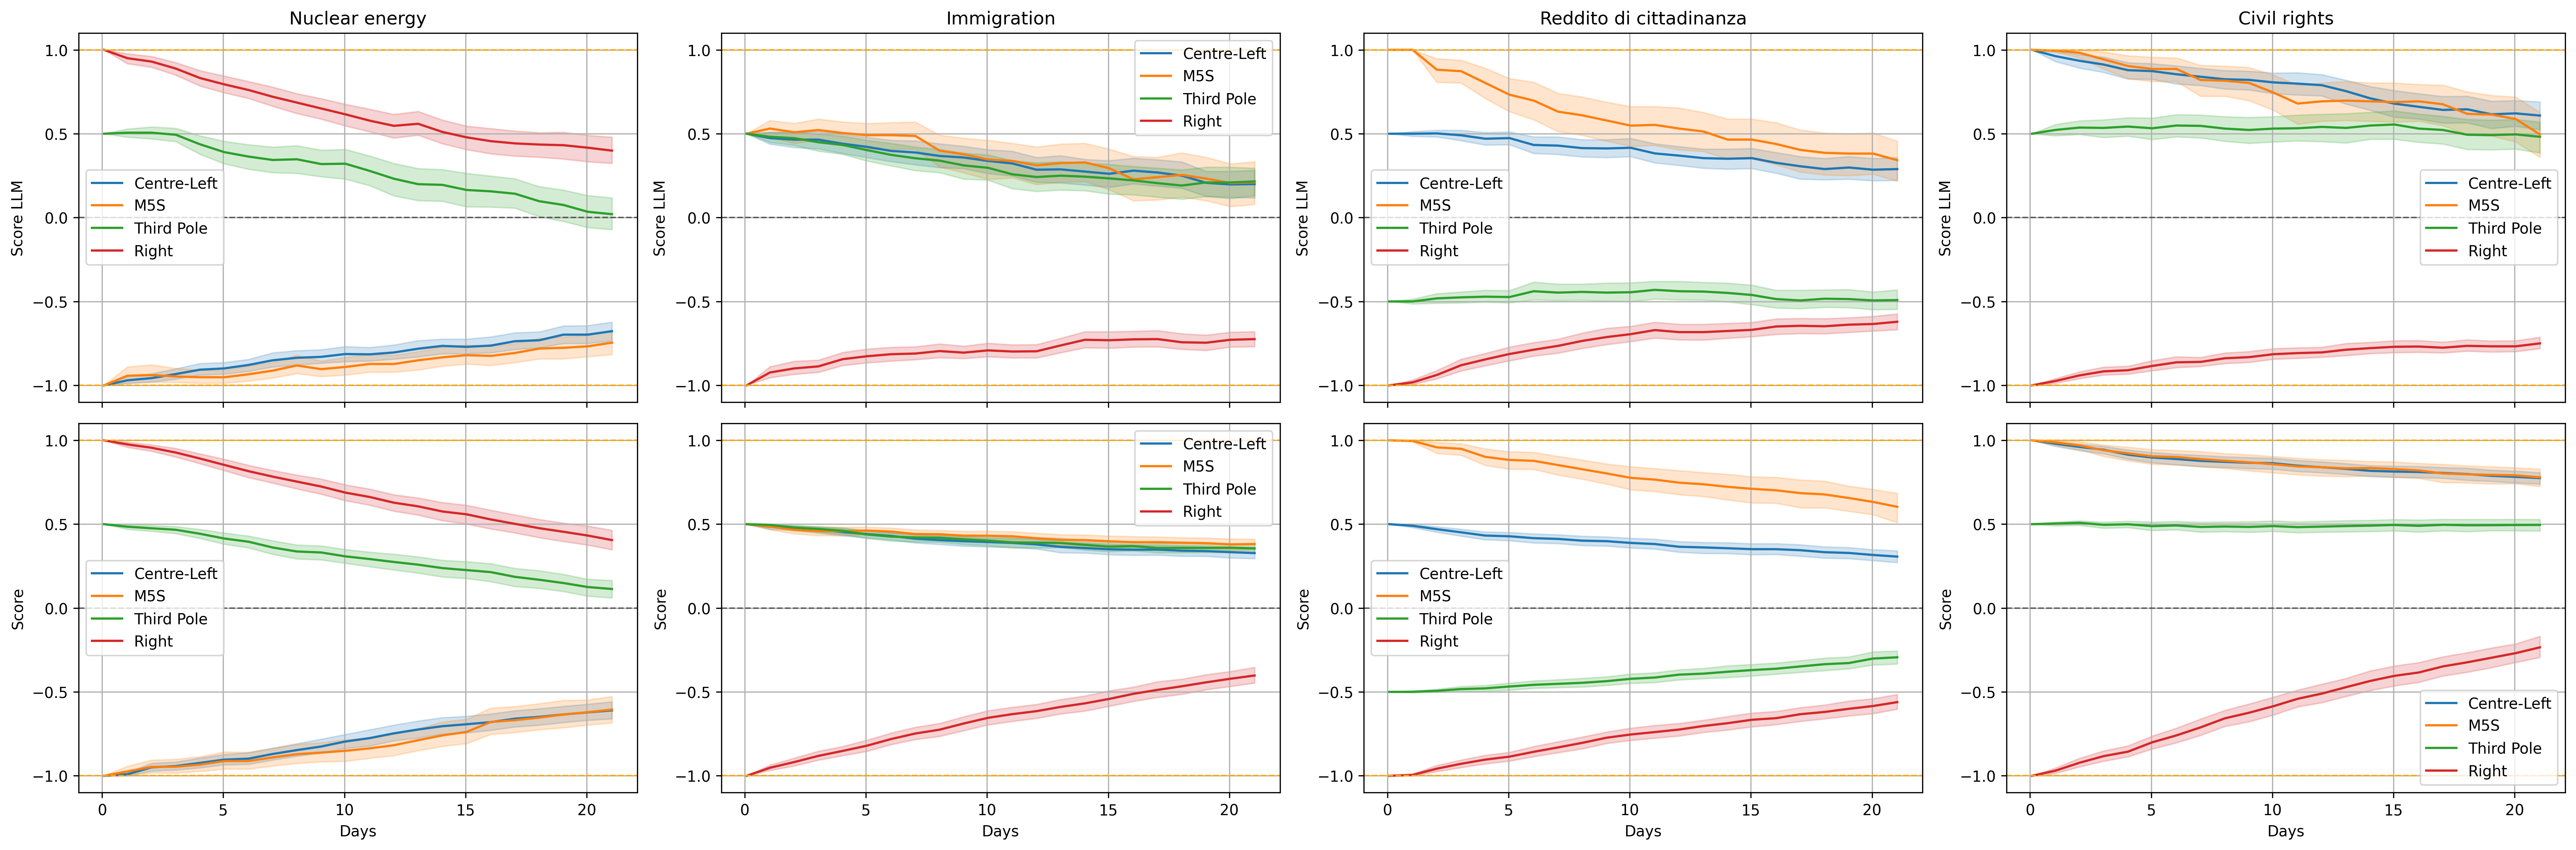
\includegraphics[width=1\linewidth]{Images/Opinions/d21a100m00d_DefaultRecSys.png}
    \caption{Evolution of opinion for each topic, comparing LLM-assigned score (\textit{score\_llm}, top row) and the one assigned by a traditional model (\textit{score}, bottom row).
    Each line represents a coalition, with a 95\% confidence interval.
    This figure is based on the runs for a single setup, but the trend is consistent with the other scenarios.}
    \label{fig:opinion_evolution}
\end{figure}


% Misinformation
\subsection{Misinformation}
% Intro, description
To analyze the impact of misinformation in the simulations, the opinion shift, defined as the difference between each user's final opinion and their initial opinion, has been considered.
Figure \ref{fig:misinfo_opinion_shift} shows, for each topic and each political coalition, the distribution of the opinion shift with different levels of misinformation.

% No effect
A clear result is that the amount of misinformation in the system doesn't cause significant changes in agents' opinions.
Even under extreme conditions, with 50\% of agents acting as misinformers, the distributions of opinion shifts overlap with those observed in the scenarios with lower or no misinformation.
This holds across all topics and political coalitions, and it means that LLM-based agents, even when exposed to large amounts of misleading content, don't have significant changes in how they update their opinions.

% Convergence to 0
Although most distributions are centered around zero, they also display asymmetries.
This reflects that agents started with different initial opinions and shifted accordingly during the simulation.
This result is consistent with what already previously discussed in Figure \ref{fig:opinion_evolution}, where opinions tend to converge toward more neutral positions over time.
However, the presence of misinformation seems not to affect the convergence process.

% Bias
A possible question is whether the lack of misinformation impact might be related to the confirmation bias, which was explicitly introduced in these work.
It's true that confirmation bias is visible in the figure: Some distributions are relatively narrow, indicating a resistance to opinion change.
However, this doesn't mean that opinions remain fixed: in several cases, distributions show shifts away from zero, indicating that agents are still able to change their views.
Nevertheless, the amount of misinformation in the environment doesn't affect the direction or the quantity of these opinion changes. Agents evolve their opinions over time, but the dynamics of change are independent from the presence of misinformation.

% Confronto coalizioni
A comparison between different coalitions highlights that the Right coalition has the narrowest distributions, centered in zero.
This suggests that supporters of this group are more resistant to change, independently from the topic and the level of misinformation.
A possible explanation is that individuals supporting the Right were initialized with stronger stances, both in the numerical scores and in the descriptions of their view. 
As a consequence, during the simulations agents tend to maintain their initial position, also supported by the confirmation bias.

% Considerazioni generali LLMs
These results highlight an important limitation: even though LLMs are effective at simulating realistic conversations, they seem not to be sensitive to the effects of misinformation, unlike real-world users \cite{aimeur2023fake}.
In real setting, people may accept false content for a variety of reasons, including emotional factors, difficulty in distinguishing true from false information, preexisting believes, or social influence signals (such as likes, shares and comments).

Even though the agents in these simulation were enriched with personality traits and confirmation bias, this was not sufficient to fully reproduce the susceptibility to misinformation observed in real-world users.
To make the simulations more realistic, it might be necessary to explicitly integrate additional psychological and social factors into the agent design, such as emotional reasoning and social validation.


\begin{figure}[h]
    \centering
    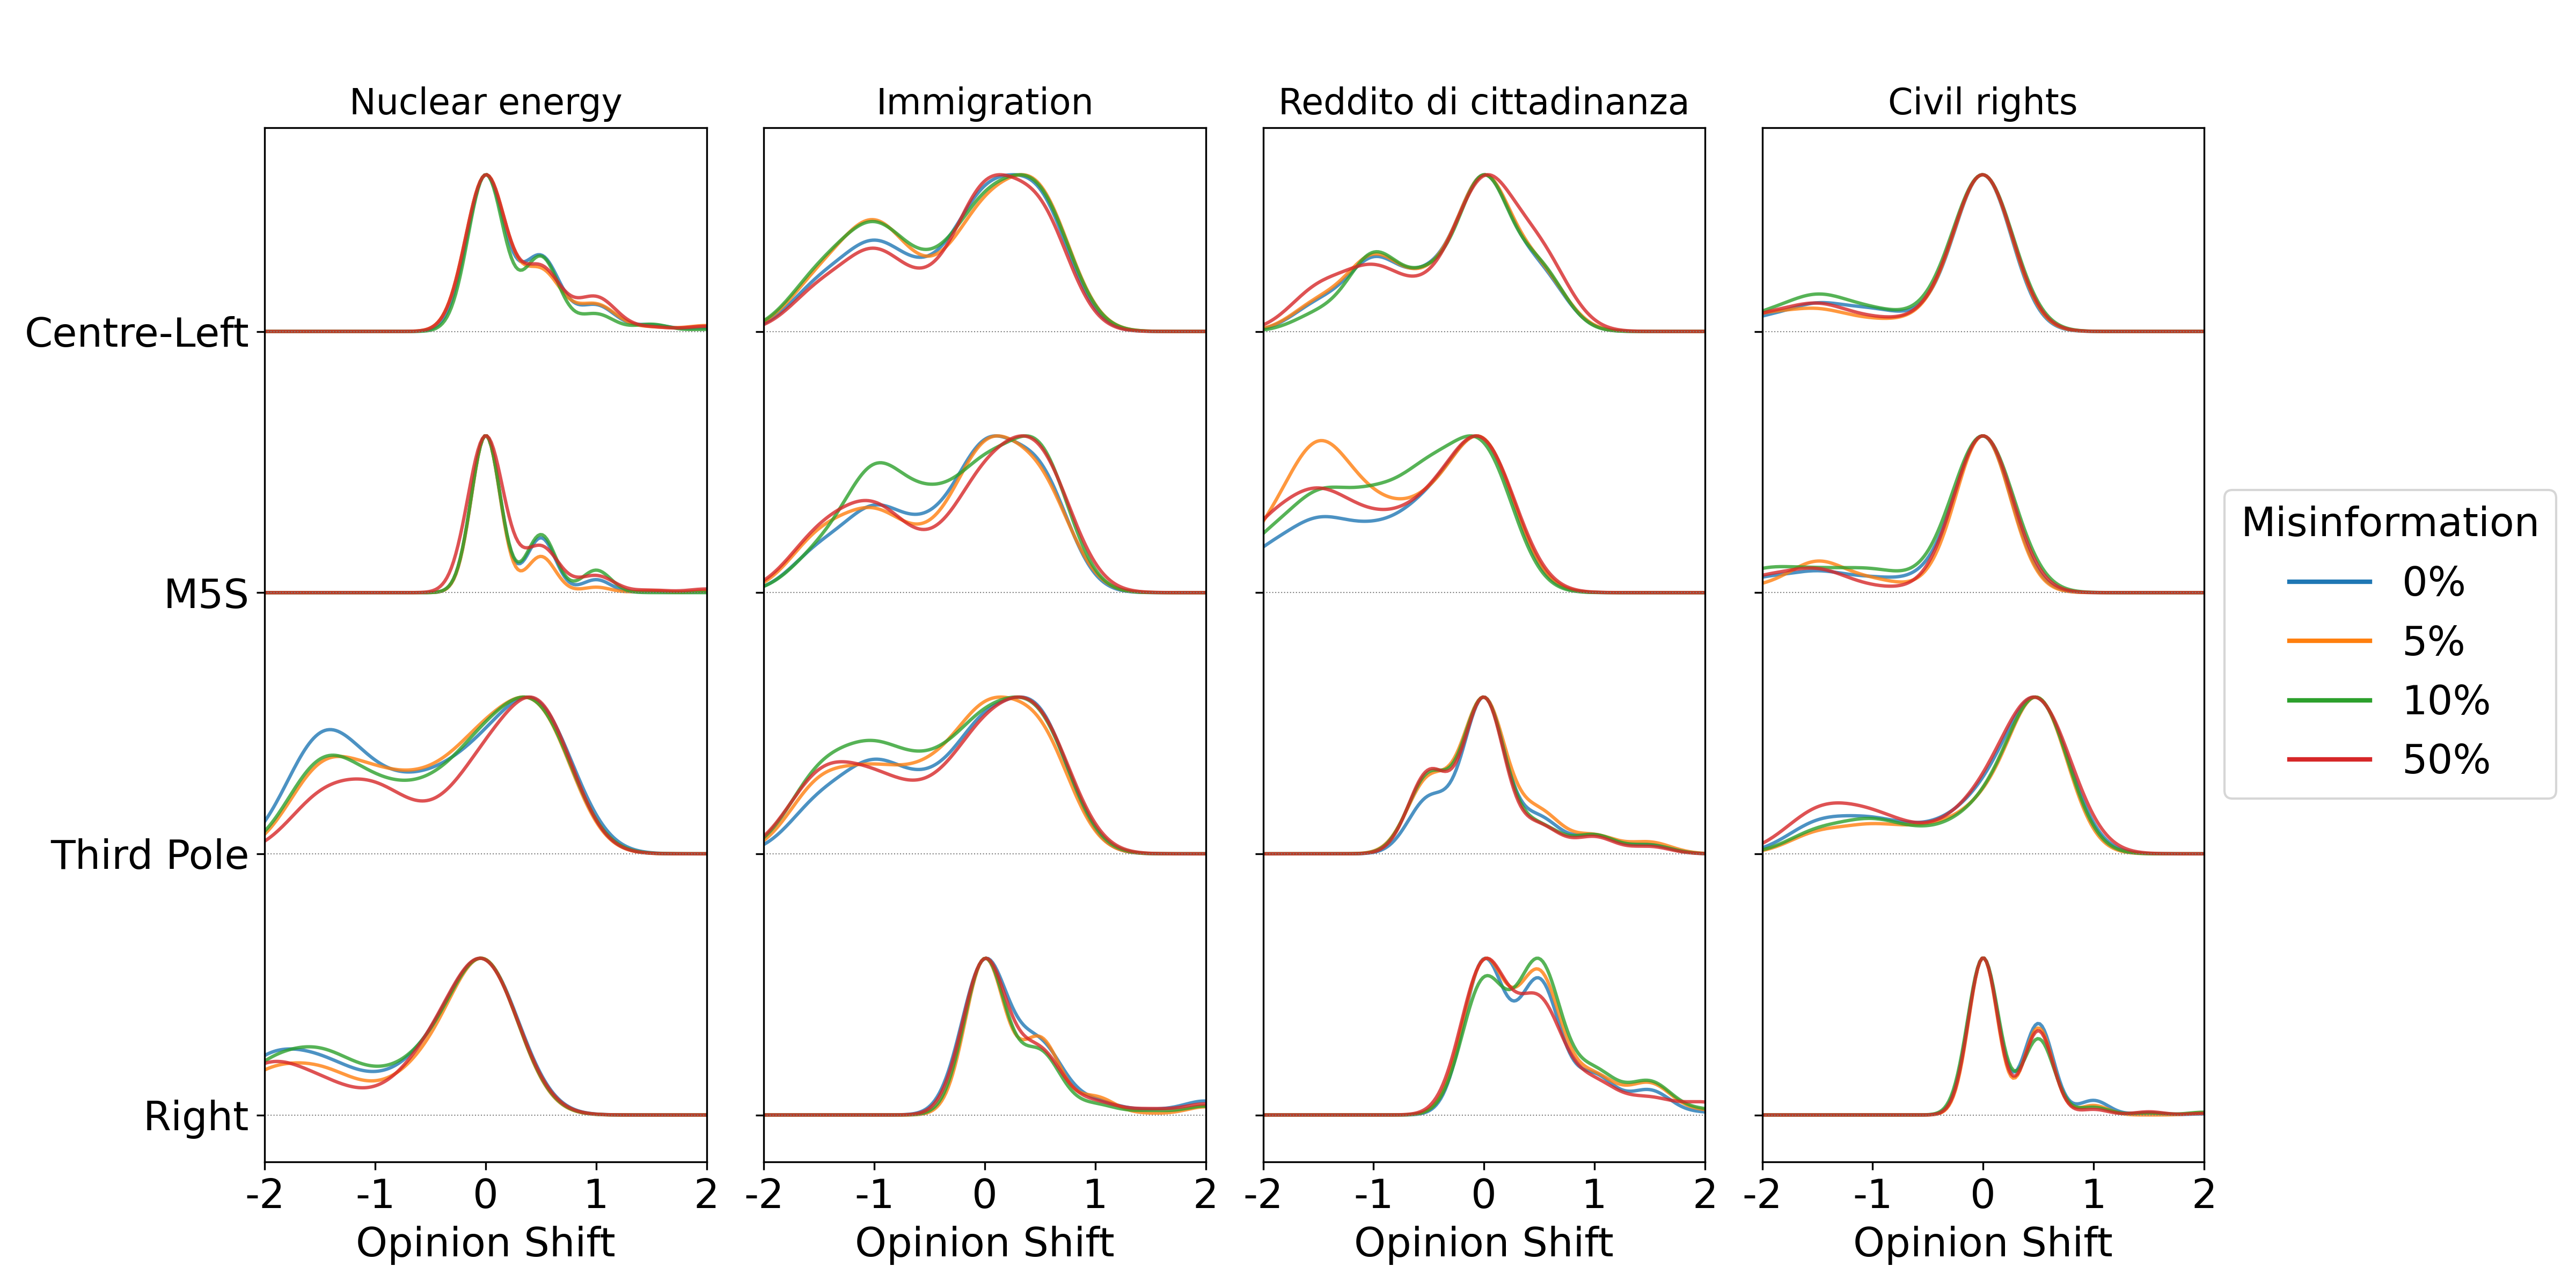
\includegraphics[width=0.8\linewidth]{Images/Misinformation/score_llm_RandomRecSys.png}
    \caption{
    Distribution of opinion shift (difference between final and initial opinion) for each topic an coalition, with varying levels of misinformation.
    The curves, which are almost completely overlapping, show that the presence of misinformation (up to 50\%) doesn't generate significant shifts in the opinions of LLM agents.
    Right coalition shows narrower distributions centered around zero, indicating greater resistance to change.
    }
    \label{fig:misinfo_opinion_shift}
\end{figure}


% Toxicity analysis
\subsection{Toxicity analysis}
To analyze the toxicity of generated content, the Detoxify library \cite{hanu2020detoxify} was used. This widely adopted tool detects offensive or harmful language in text and provides a continuous toxicity score between 0 and 1.
This section explores two aspects of the toxicity in the simulations: how it varies depending on whether users interact with in-group or out-group users, and how it differs across political coalitions and content types.

\subsection{Toxicity Toward In-Group vs Out-Group}
To analyze the toxicity of comments, for each user we computed the difference between the average toxicity of replies to users from the same coalition (in-group) and those directed at users from different coalitions (out-group).
The resulting distribution is visible in Figure \ref{fig:toxicity_in_out}.
To improve readability, toxicity values were normalized according to a logarithmic scale, since original values follow an exponential distribution: $log(toxicity + 1)$.

Looking at the plot, we can see that both distributions, one for the simulated content and one for the real data, are centered around zero.
This suggests that, on average, users don't show a strong difference in behavior when replying to in-group or out-group members.

However, the distribution of the simulated data is narrower and concentrated near zero.
This means that most agents behave in a similar way, with small variations in the toxicity difference between groups.

In contrast, the real data show a wider distribution: some users are more hostile way toward other coalitions, while others show more toxic behavior toward people supporting the same coalition.
This indicates a greater variety of behaviors in real-world interactions.

It's also possible to notice that both curves have a slight shift to the right, which may suggest a slight tendency to be more toxic toward out-group members. However, this effect is minimal.

Overall, the simulations fail to reproduce the diversity of behaviors observed in real data. 
In the scenarios studies, LLMs tend to behave in a uniform way and are not able to capture the differences in hostility toward different groups.


\begin{figure}[h]
    \centering
    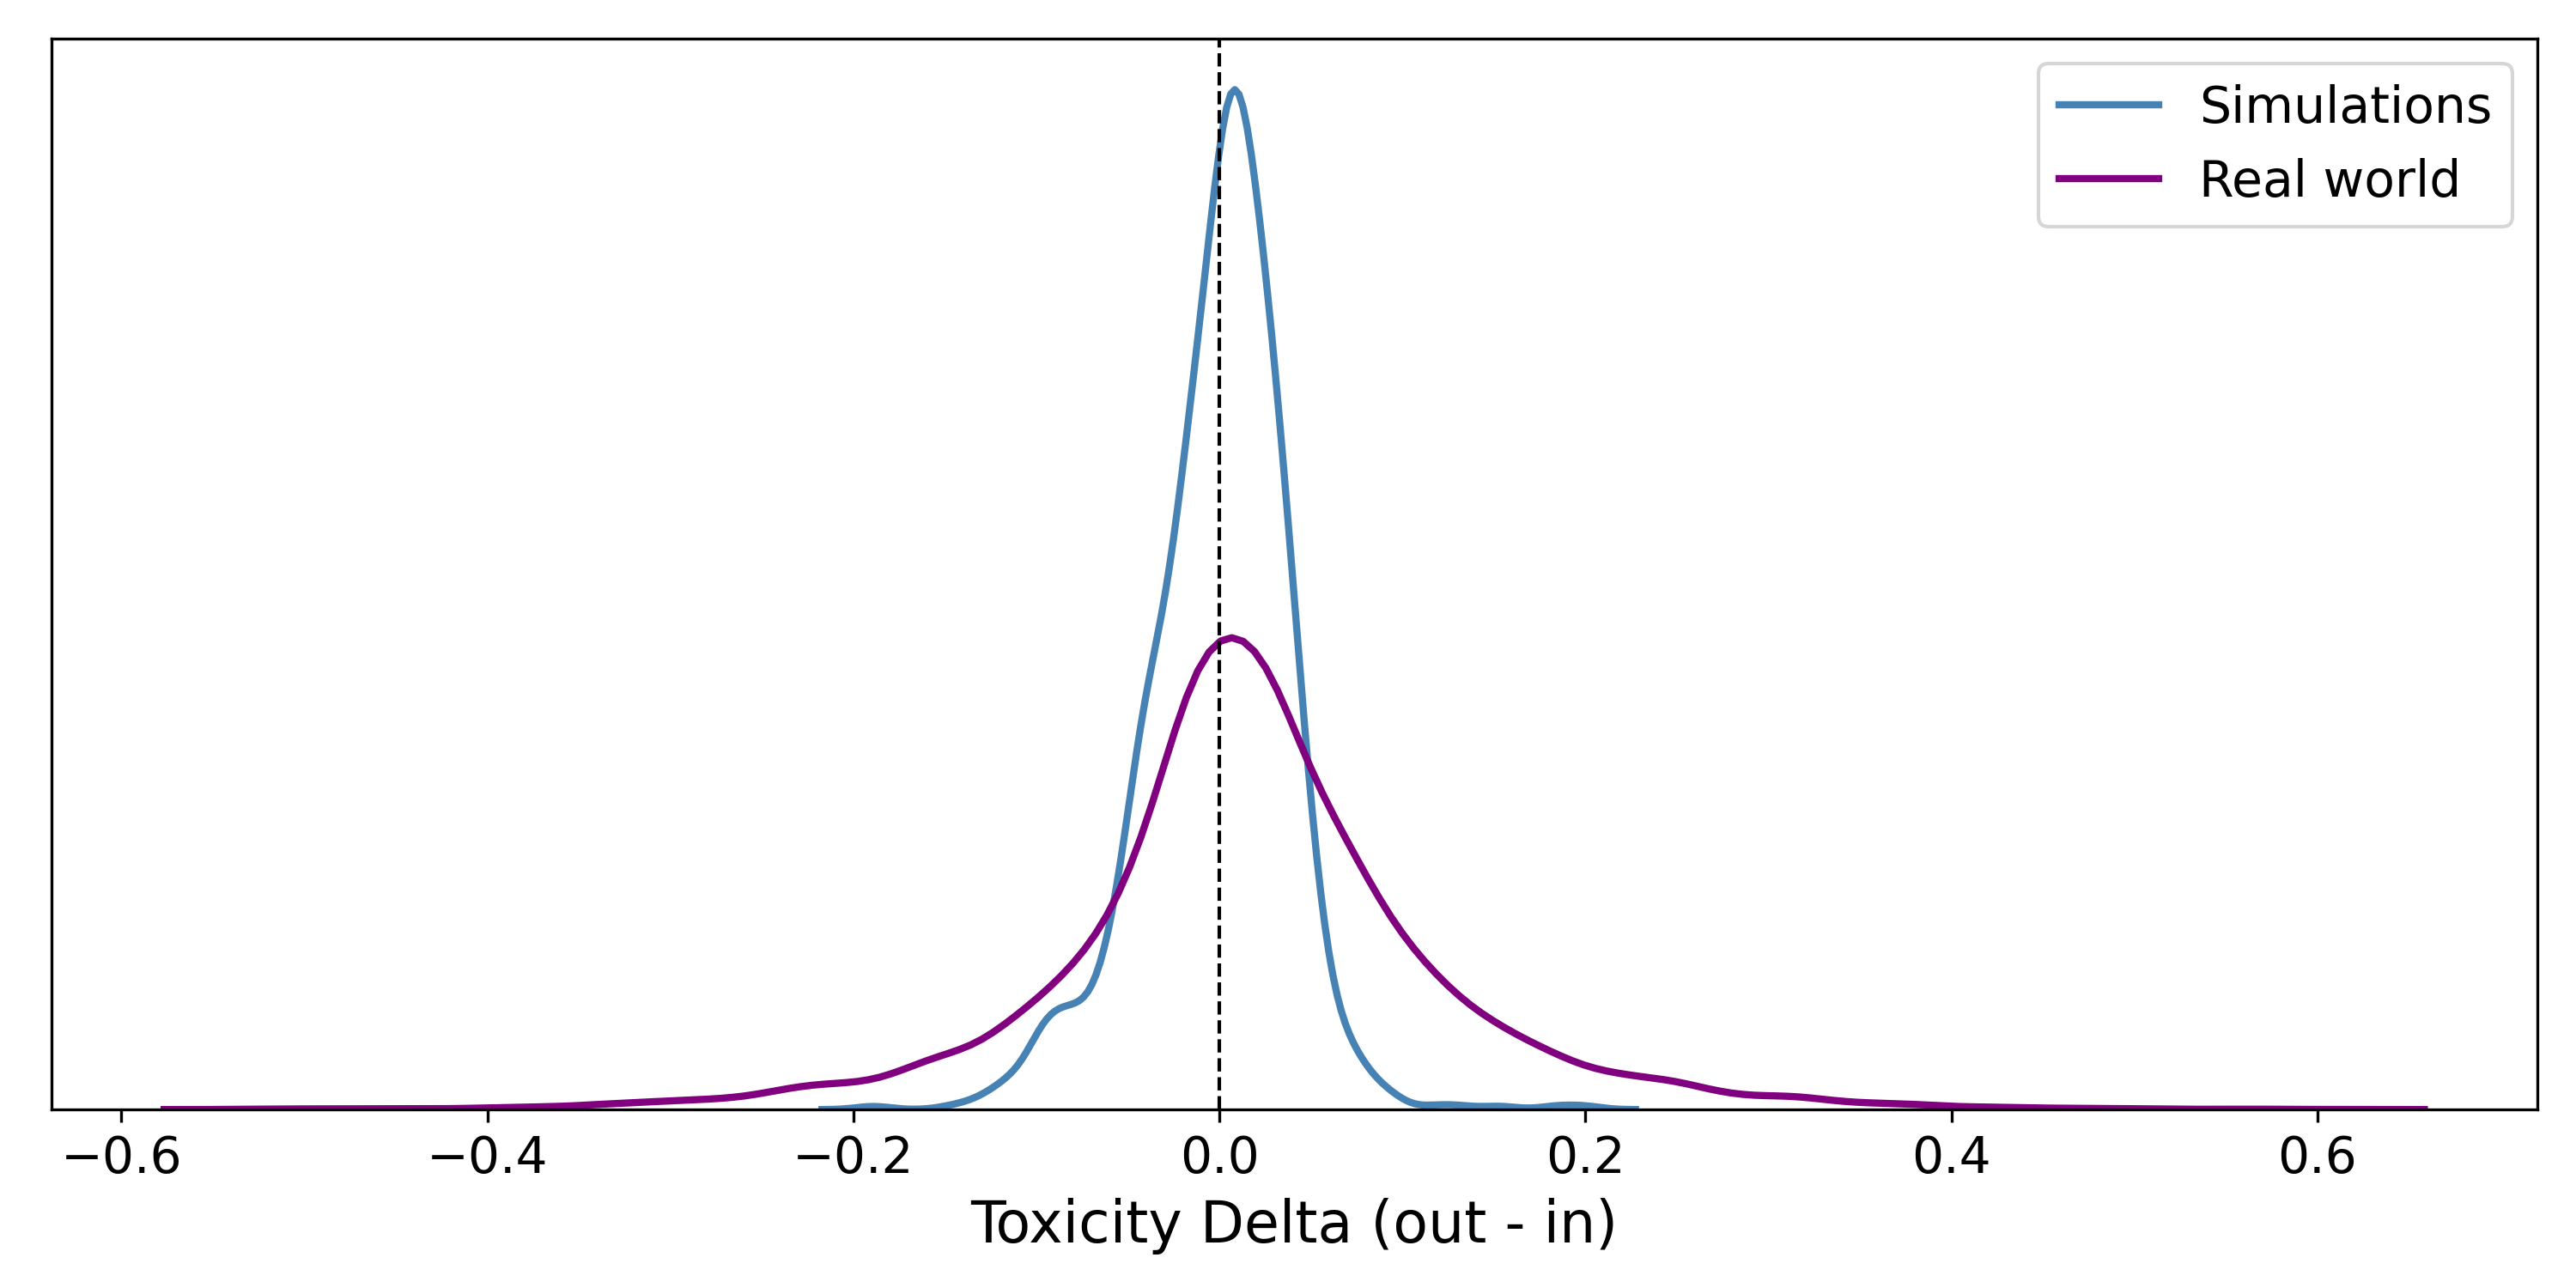
\includegraphics[width=0.6\linewidth]{Images/Toxicity/diff_in_out_combined.png}
    \caption{
    Distribution of the difference in mean toxicity toward out-group and in-group in user comments.
    The distribution of simulated content is more centered and narrow, indicating that agents behave similarly across groups.
    Real-wold data show greater variance, suggesting that some users are more hostile toward one of the two groups.
    }
    \label{fig:toxicity_in_out}
\end{figure}


\subsection{Toxicity Across Coalitions and Content Types}
The analysis of toxicity in texts generated by LLMs, divided by post and comments and categorized by political coalition, is visible in Figure \ref{fig:toxicity_box}, and reveals some interesting dynamics in the communication style of the agents within the simulations.

In general, posts tend to be more toxic on average than comments, with an a single exception: the Right coalition.
In this case, the generated comments are more toxic than the posts, suggesting that the the Right tends to bring more conflictual contributions to the conversations.
The Right coalition also shows the greatest variance in comment toxicity.
This suggests that their replies are more heterogeneous and can include extremely toxic texts.

The M5S coalition exhibits the greatest average toxicity in posts.
In addition, the distribution shows a visible positive skew, indicating that, beyond the generally more aggressive tone, there are also occasional posts with high levels of toxicity.

In contrast, the Centre-Left and Third Pole coalitions maintain a more moderate and stable tone, across both comments and posts.

Another important insight from this analysis concerns the shape of the toxicity distribution.
In all cases, the data shows a relevant positive skew: most texts have very low toxicity, but there are long tails extending toward higher values.
This pattern becomes particularly evident when using a logarithmic scale on the y axis, which makes these cases more visible.
This suggests that, despite the generally low average toxicity, LLMs can still produce highly toxic content, even though at lower frequency.

This ability to generate even highly toxic texts, maybe facilitated by the use of an uncensored language model, is beneficial in the context of social media simulations, as it allows a more realistic modeling of online conversations.


\begin{figure}[h]
    \centering
    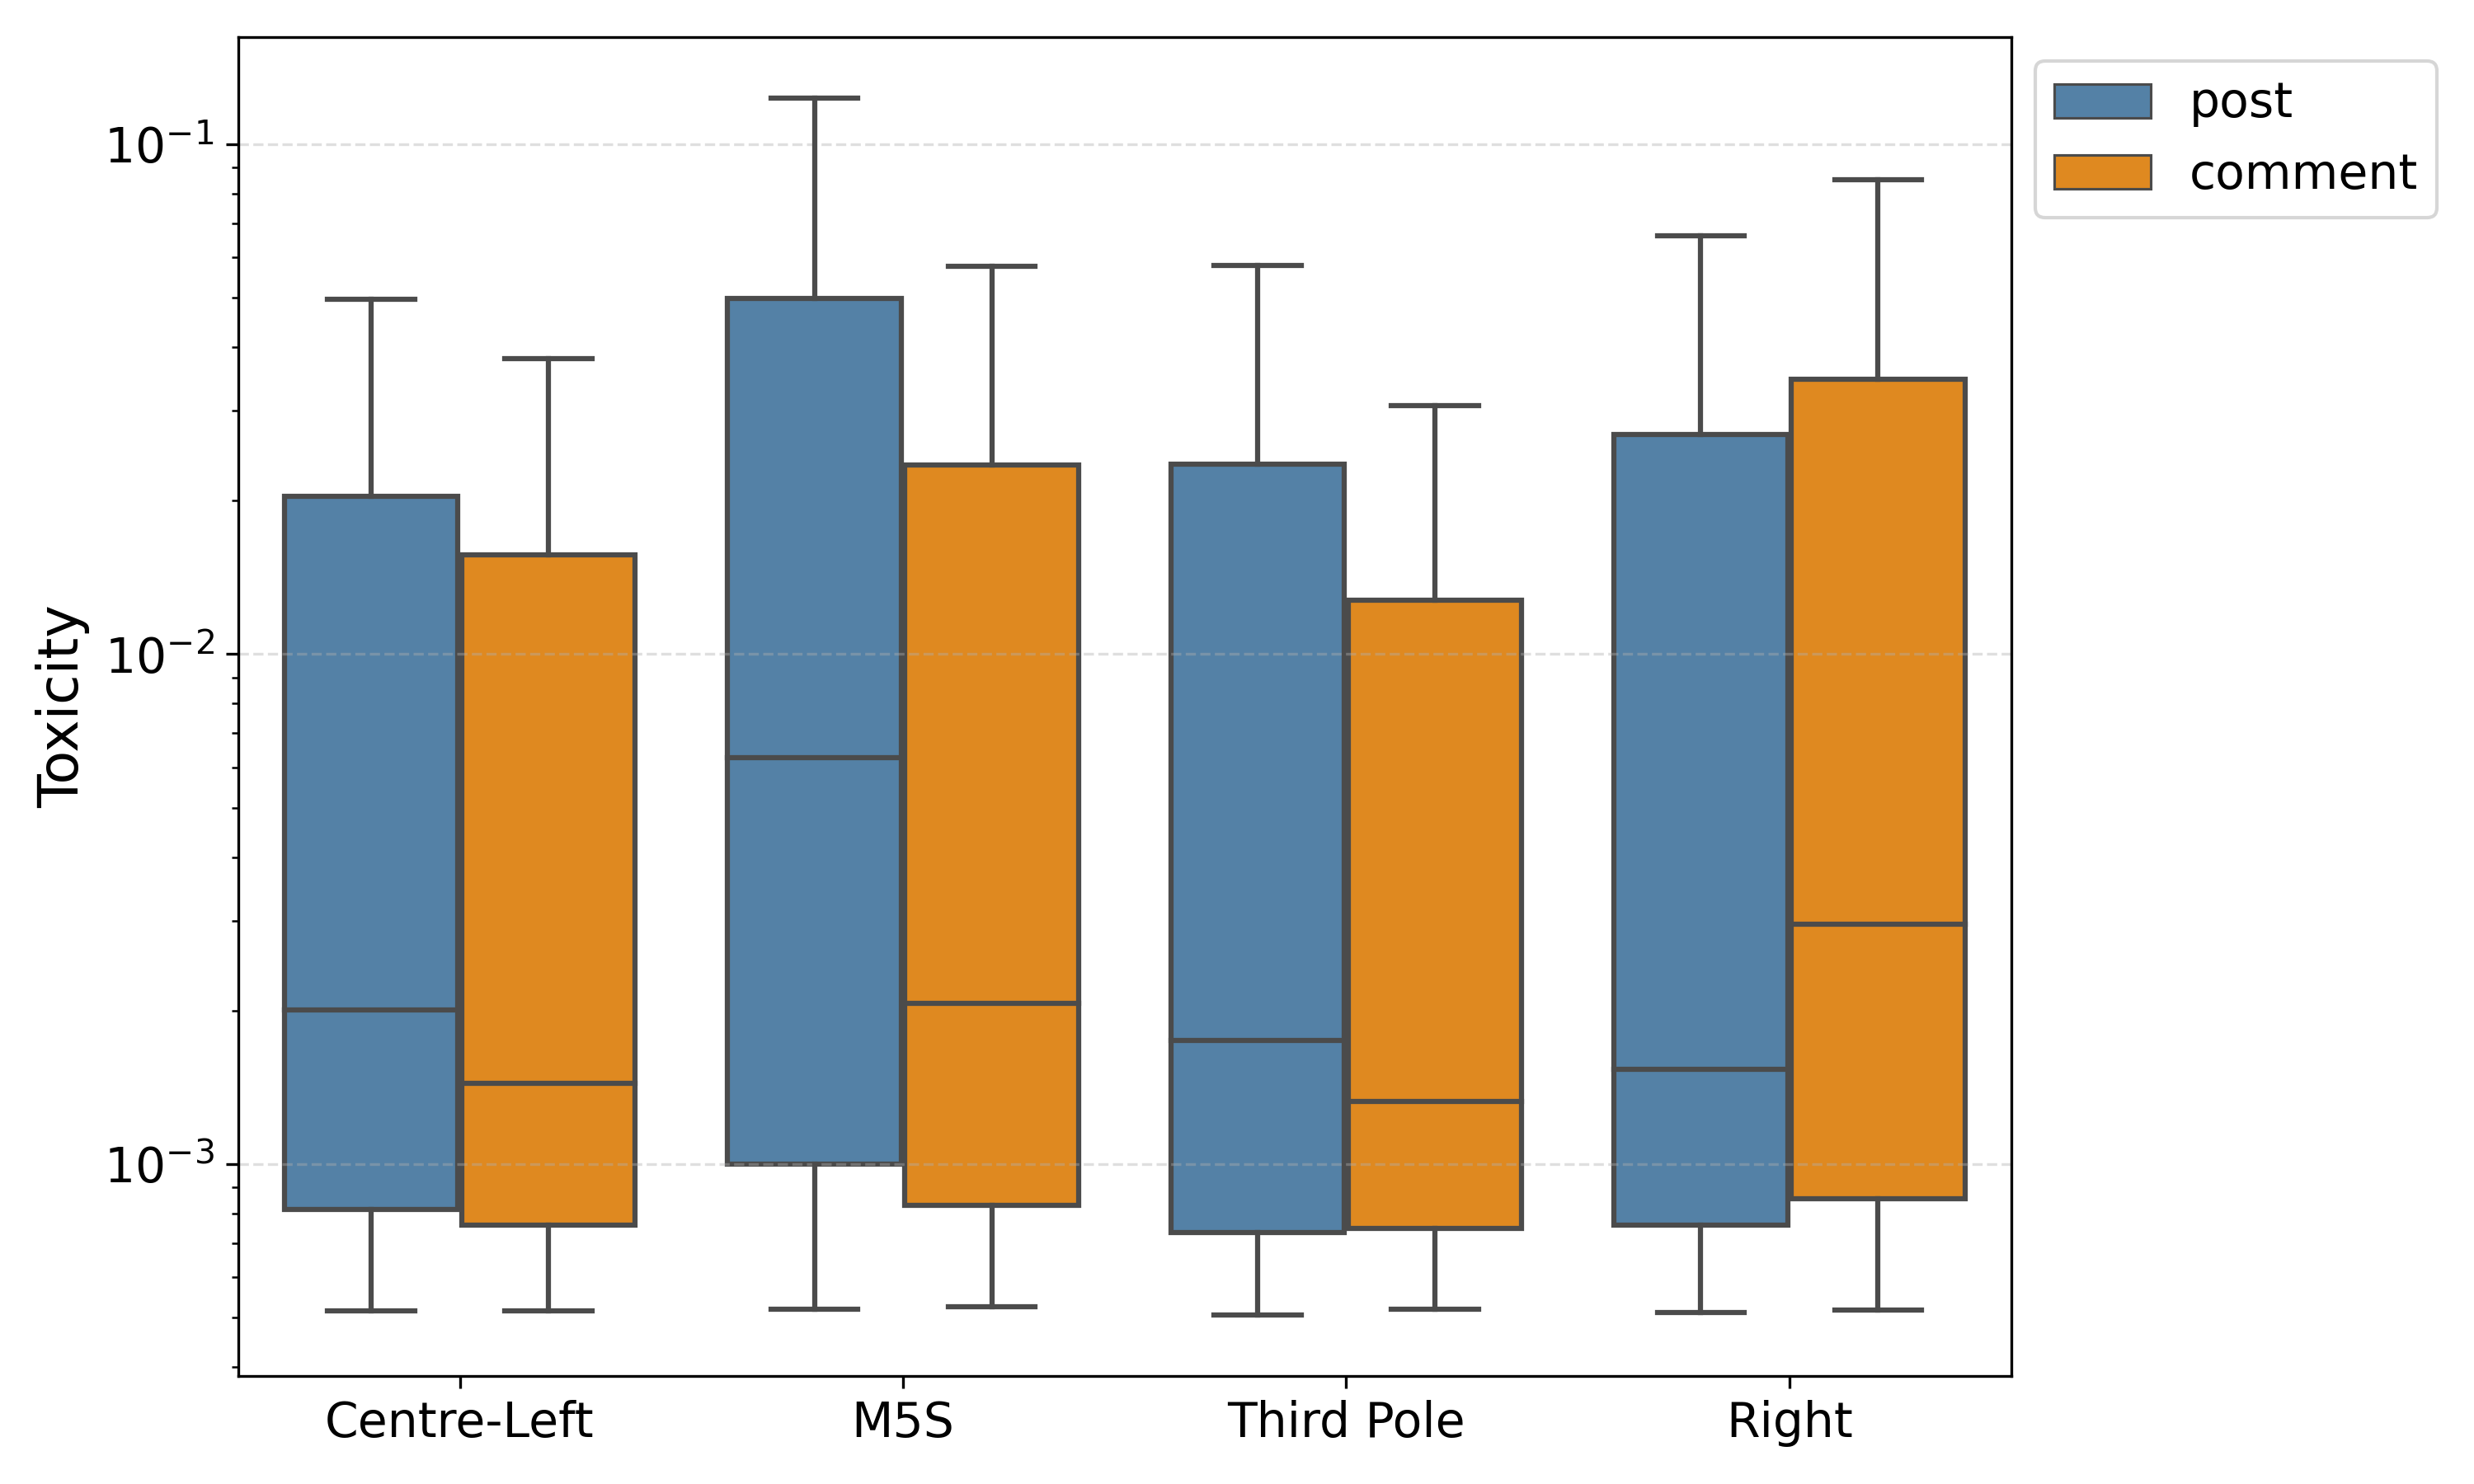
\includegraphics[width=0.6\linewidth]{Images/Toxicity/box_posts_vs_comments.png}
    \caption{
    Toxicity of LLM-generated texts, in posts and comments per political coalition.
    The y axis is in logarithmic scale to highlight the skew of the distribution.
    The Centre-Left and Third Pole coalitions have more stable and moderate tones.
    M5S is the most toxic in posts, while the Right generates comments with greater variability and toxicity.
    The long tails in all cases indicate that LLMs can generate content extremely toxic, even if rarely.
    }
    \label{fig:toxicity_box}
\end{figure}


% Recsys
\subsection{Content Recommendation Algorithms}
A comparison of the two content recommendation algorithms on the previously presented plots doesn't highlight any significant difference.
This happens because, at the beginning of the simulation, agents are not connected, so the network is empty.
Therefore, the used recommended system, \textit{ReverseChronoFollowersPopularity}, which should promote popular content from followers, doesn't have enough information to provide the best content.
In this initial phase, its behavior is similar to \textit{ContentRecSys}, the algorithm that suggests random content.

As a result, the different effects of the recommendation systems cannot emerge in the first few virtual days, and the dynamics produced by the two approaches are the same.
To see a real impact of the different recommender systems, simulations should run on a longer virtual time, or a network should be initialized with preexisting connections, providing a complete context of the initial user preferences.

This would allow a better evaluation of the impact of content selection on social networks.
\section{Conclusions}
\label{sec:conclusions}

% Goal
Large Language Models (LLMs) have emerged as a promising tool to simulate agents in virtual environments. 
The main goal of this work is to analyze the behavior of LLM-based agents in the context of online social media platforms.
For this reason, the \textit{Y} simulator has been extended to integrate mechanisms for opinion evolution, the presence of misinformation agent,s and a realistic user initialization based on real-world data from the 2022 Italian political context.

% Analyses
\medskip
To explore the simulated agents from multiple perspectives, the analysis has been conducted at different levels: from the structure of the social graph, to the types of interactions, the evolution of opinions, and the toxicity of generated content.

The results show that LLMs are a promising approach for simulating realistic behavior. Agents are capable of interacting, forming connections, and generating content with varying toxicity, even though they tend to favor neutral tones.

% Limitations
\medskip
However, some limitations of this work emerged.
In particular, the impact of misinformation appeared negligible: even in scenarios where many agents shared misleading content, opinion dynamics remained unaffected.
This suggests that LLM agents are not sensitive to misleading information in the way real users are.
A possible reason is that the agent profiles, although already enriched with personality traits and confirmation bias, are not sufficient to represent more complex behaviors.
A more detailed initialization, for instance including emotional responses, susceptibility to influence, or trust of the information they read, might allow more realistic dynamics to emerge.

\medskip
Another limitation concerns the duration of the simulations. 
The 21 simulated days were enough for a network structure to emerge, but not long enough to observe meaningful long-term evolution.
For instance, actions such as \textit{unfollow} are almost absent, and the effect of the different content recommendation systems did not emerge, since the network was not yet sufficiently structured in the first virtual days.

As for opinion evolution, the scores assigned by LLMs were consistent with those of traditional models, both tending to converge toward neutral positions. 
Even in this case, running longer simulations might reveal whether these trends tend to stabilize or diverge over time.

% Conclusion
\medskip
In conclusion, integrating LLMs as agents in social simulations represent a significant step toward more realistic modeling, especially in terms of language, interactions, and content generation.
However, to replicate more heterogeneous phenomena, such as the spread of misinformation, further work is needed to enrich the agents' behavioral models.

This research direction supports the exploration of increasingly realistic simulations, enabling the investigation of complex social dynamics under controlled conditions. 

\newpage


% BIBLIOGRAPHY
%\section{Bibliography and citations}

% BIBLIOGRAPHY
\bibliography{bibliography.bib}

\appendix
\section{Appendix A}
If you need to include an appendix to support the research in your thesis, you can place it at the end of the manuscript.
An appendix contains supplementary material (figures, tables, data, codes, mathematical proofs, surveys, \dots)
which supplement the main results contained in the previous sections.

%%%%%%%%%%%%%%%%%%%%%%%%%%%%%%%%%%%%%%%%%%%%%%%%%%%%%%%%%%%%%%
%%     ABSTRACT IN ITALIAN LANGUAGE AND ACKNOWLEDGMENTS     %%
%%%%%%%%%%%%%%%%%%%%%%%%%%%%%%%%%%%%%%%%%%%%%%%%%%%%%%%%%%%%%%
\cleardoublepage

% SOMMARIO
\section*{Abstract in lingua italiana}
Qui va l'Abstract in lingua italiana della tesi seguito dalla lista di parole chiave.
\vspace{15pt}
\begin{tcolorbox}[arc=0pt, boxrule=0pt, colback=bluePoli!60, width=\textwidth, colupper=white]
    \textbf{Parole chiave:} qui, le parole chiave, della tesi, in italiano 
\end{tcolorbox}

% ACKNOWLEDGEMENTS
\section*{Acknowledgements}
Here you might want to acknowledge someone.

%%%%%%%%%%%%%%%%%%%%%%%%%%%%%%%%%%
%%     END OF YOUR DOCUMENT     %%
%%%%%%%%%%%%%%%%%%%%%%%%%%%%%%%%%%
\end{document}